% ============================================================
% 2.2 Existing Approaches
% ============================================================

\section{Approaches}
\label{sec:sota_approaches}

% The requirements defined in Section~\ref{sec:requirements_analysis}
% describe the capabilities expected from a solution for secure
% AI-driven DeFi execution. This section reviews existing approaches
% that address different parts of these requirements. The literature
% is organised into five \textit{approach groups}, according to the
% main technical focus considered in the discussion:
% execution control, AI-assisted action generation, knowledge
% retrieval, graph-based relationship analysis, and smart-contract
% security analysis.

% These groups provide a structure for the review rather than a
% classification into mutually exclusive types of systems. They
% cover both technical mechanisms and analytical objectives.
% A single system may therefore contribute to more than one group.
% For example, a smart-contract security tool may use a graph to
% represent function calls or data dependencies. Its graph
% representation is relevant to graph-based relationship analysis,
% while its investigation of vulnerabilities is relevant to
% smart-contract security analysis. The distinction between these two groups concerns the aspect
% being examined. Graph-based relationship analysis focuses on
% how connected information is represented, queried, or analysed.
% Smart-contract security analysis focuses on whether contract
% code or behaviour exhibits vulnerabilities or violates specified
% properties. Their overlap does not make them interchangeable.
% Where a system is discussed in both groups, each discussion
% addresses the aspect relevant to that group.

% Individual standards, frameworks, and research systems are
% examined as representative examples. For each group, the review
% considers the information processed, the mechanism applied,
% the result produced, and its relevance to the requirements.
% It distinguishes capabilities demonstrated by the reviewed
% systems from capabilities that depend on additional components.
% A practical solution may combine several groups, such as
% AI-assisted intent generation, relationship verification,
% and execution controls.

% Table~\ref{tab:approach_groups} summarises the focus of each group.
% The requirement comparison in Section~\ref{sec:sota_comparison}
% assesses their coverage of R1--R6. Similar ratings indicate
% similar coverage under the assessment criteria; they do not
% imply that the approaches have the same purpose or are
% technically equivalent.


The requirements defined in Section~\ref{sec:requirements_analysis}
describe the capabilities expected from a solution for secure
AI-driven DeFi execution. This section reviews existing approaches
that address different parts of these requirements. The literature
is organised into five \textit{approach groups} according to their
primary technical focus: execution control, AI-assisted blockchain
action generation, knowledge retrieval, graph-based relationship
analysis, and smart-contract security analysis.

Each approach group represents a broad technical direction. Within
these groups, subgroups distinguish methods according to their
underlying mechanisms or analytical objectives. Individual
standards, frameworks, and research systems are discussed as
representative examples of the corresponding methods. This
distinction is important because the capabilities demonstrated by
one system do not necessarily apply to every approach within
the same group.

The groups are not mutually exclusive. A system may combine
mechanisms from several groups or be relevant to more than
one analytical objective. For example, smart-contract security
analysis may use graphs to represent function calls or data
dependencies. Such representations are relevant to graph-based
relationship analysis, while the identification of vulnerabilities
belongs to smart-contract security analysis. The distinction
therefore concerns the purpose for which a mechanism is used,
rather than the presence of a particular technology. For each group, the review first considers its general
characteristics, including the information processed, the
mechanisms applied, and the results produced. The subsequent
discussion examines the relevant subgroups and representative
systems, including their contributions and limitations with
respect to the requirements. Capabilities inherent to a method
are distinguished from those demonstrated by individual
implementations or requiring additional components.

Figure~\ref{fig:approach_hierarchy} provides an overview of
the reviewed approach groups and their subgroups.
Table~\ref{tab:approach_groups} summarises the technical focus
of each group. The requirement
comparison in Section~\ref{sec:sota_comparison} assesses their
coverage of R1 to R6. Similar ratings indicate similar coverage
under the assessment criteria; they do not imply that the
approaches have the same purpose or are technically equivalent.



\begin{table}[H]
\centering
\small
\renewcommand{\arraystretch}{1.15}
\begin{tabular}{p{4.8cm} p{9.2cm}}
\hline
\textbf{Approach Group} & \textbf{Focus of the Review} \\
\hline

Execution-Layer Security and Policy Enforcement &
Mechanisms that authorise or block prepared operations and
restrict the execution authority available to an account
or automated agent. \\

AI-Agent Blockchain Execution &
Methods that translate natural-language goals into structured
actions, tool calls, workflows, and blockchain operations. \\

Knowledge Retrieval and Grounding &
Methods that obtain external information to support
interpretation, planning, analysis, or verification. \\

Graph-Based Relationship Analysis &
Methods that represent and examine connected information,
including transaction flows, program dependencies, domain
knowledge, and validation dependencies. \\

Smart Contract Security Analysis &
Methods that examine contract code, execution behaviour,
and cross-contract interactions for vulnerabilities or
violations of specified properties. \\

\hline
\end{tabular}
\caption{Technical focus of the five approach groups reviewed.}
\label{tab:approach_groups}
\end{table}

\begin{figure}[H]
\centering
\begingroup

\definecolor{stepfill}{HTML}{F8FAFC}
\definecolor{stepborder}{HTML}{475569}
\definecolor{arrowcol}{HTML}{64748B}
\definecolor{steptext}{HTML}{1E293B}

\resizebox{0.98\linewidth}{!}{%
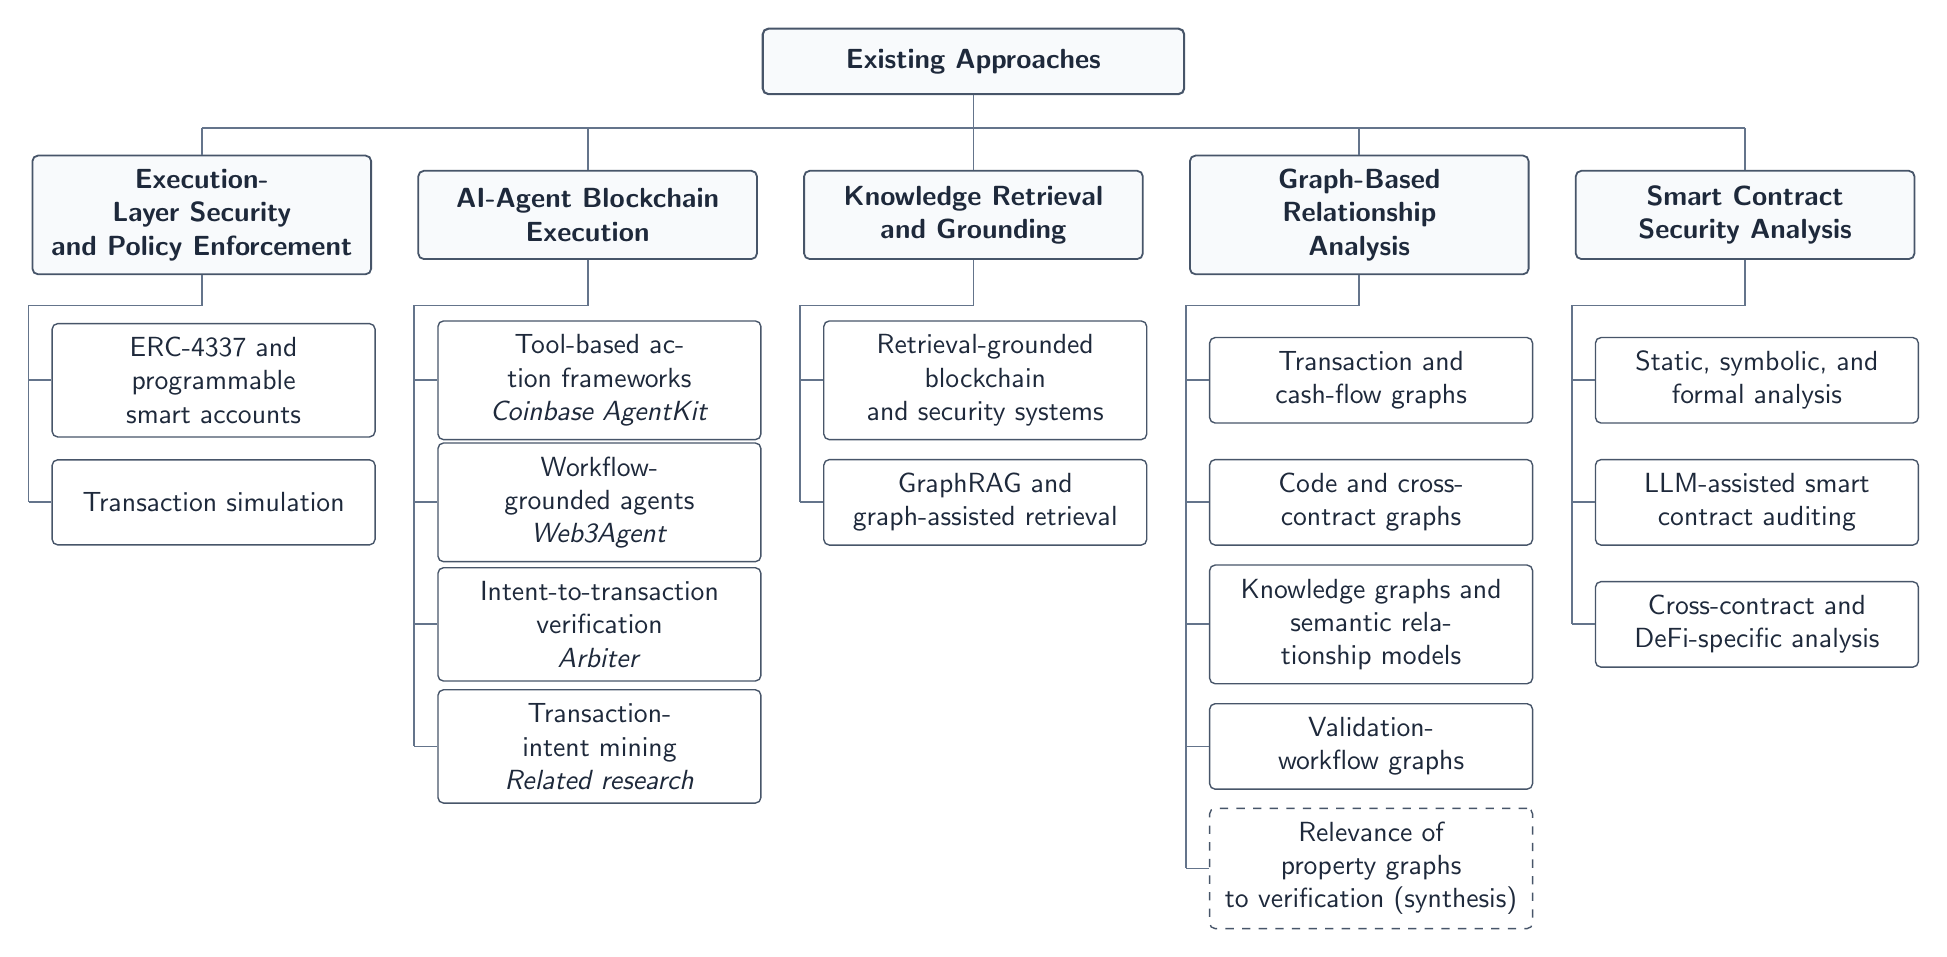
\begin{tikzpicture}[
    x=1cm, y=1cm,
    root/.style={
        draw=stepborder,
        fill=stepfill,
        rounded corners=2pt,
        line width=0.75pt,
        text=steptext,
        text width=5cm,
        minimum height=0.83cm,
        align=center,
        inner sep=5pt,
        font=\sffamily\bfseries
             \fontsize{10}{12}\selectfont
    },
    group/.style={
        draw=stepborder,
        fill=stepfill,
        rounded corners=2pt,
        line width=0.65pt,
        text=steptext,
        text width=3.95cm,
        minimum height=1.12cm,
        align=center,
        inner sep=5pt,
        font=\sffamily\bfseries
             \fontsize{10}{12}\selectfont
    },
    subgroup/.style={
        draw=stepborder,
        fill=white,
        rounded corners=2pt,
        line width=0.5pt,
        text=steptext,
        text width=3.75cm,
        minimum height=1.08cm,
        align=center,
        inner xsep=5pt,
        inner ysep=5pt,
        font=\sffamily
             \fontsize{10}{12}\selectfont
    },
    synthesis/.style={
        subgroup,
        dashed
    },
    link/.style={
        draw=arrowcol,
        line width=0.65pt
    }
]

% =====================================================
% LEVEL 1: ROOT
% =====================================================

\node[root] (root) at (0,0)
    {Existing Approaches};


% =====================================================
% LEVEL 2: FIVE APPROACH GROUPS
% =====================================================

\node[group] (g1) at (-9.8,-1.95)
    {Execution-Layer Security\\
     and Policy Enforcement};

\node[group] (g2) at (-4.9,-1.95)
    {AI-Agent Blockchain\\
     Execution};

\node[group] (g3) at (0,-1.95)
    {Knowledge Retrieval\\
     and Grounding};

\node[group] (g4) at (4.9,-1.95)
    {Graph-Based Relationship\\
     Analysis};

\node[group] (g5) at (9.8,-1.95)
    {Smart Contract\\
     Security Analysis};


% =====================================================
% ROOT-TO-GROUP BRANCHES
% =====================================================

\draw[link]
    (root.south) -- (0,-0.85);

\draw[link]
    (-9.8,-0.85) -- (9.8,-0.85);

\foreach \n in {1,2,3,4,5} {
    \draw[link]
        (g\n.north) --
        (g\n.north |- 0,-0.85);
}


% =====================================================
% LEVEL 3: GROUP 1
% Execution-Layer Security and Policy Enforcement
% =====================================================

\node[subgroup] (a1) at (-9.65,-4.05)
    {ERC-4337 and\\
     programmable smart accounts};

\node[subgroup] (a2) at (-9.65,-5.60)
    {Transaction simulation};


% =====================================================
% LEVEL 3: GROUP 2
% AI-Agent Blockchain Execution
% =====================================================

% Individual systems are representative examples.

\node[subgroup] (b1) at (-4.75,-4.05)
    {Tool-based action frameworks\\
     \textit{Coinbase AgentKit}};

\node[subgroup] (b2) at (-4.75,-5.60)
    {Workflow-grounded agents\\
     \textit{Web3Agent}};

\node[subgroup] (b3) at (-4.75,-7.15)
    {Intent-to-transaction verification\\
     \textit{Arbiter}};

\node[subgroup] (b4) at (-4.75,-8.70)
    {Transaction-intent mining\\
     \textit{Related research}};


% =====================================================
% LEVEL 3: GROUP 3
% Knowledge Retrieval and Grounding
% =====================================================

\node[subgroup] (c1) at (0.15,-4.05)
    {Retrieval-grounded blockchain\\
     and security systems};

\node[subgroup] (c2) at (0.15,-5.60)
    {GraphRAG and\\
     graph-assisted retrieval};


% =====================================================
% LEVEL 3: GROUP 4
% Graph-Based Relationship Analysis
% =====================================================

\node[subgroup] (d1) at (5.05,-4.05)
    {Transaction and\\
     cash-flow graphs};

\node[subgroup] (d2) at (5.05,-5.60)
    {Code and cross-contract graphs};

\node[subgroup] (d3) at (5.05,-7.15)
    {Knowledge graphs and\\
     semantic relationship models};

\node[subgroup] (d4) at (5.05,-8.70)
    {Validation-workflow graphs};

% The final box represents a synthesis, not
% a separate approach subgroup.

\node[synthesis] (d5) at (5.05,-10.25)
    {Relevance of property graphs\\
     to verification (synthesis)};


% =====================================================
% LEVEL 3: GROUP 5
% Smart Contract Security Analysis
% =====================================================

\node[subgroup] (e1) at (9.95,-4.05)
    {Static, symbolic, and\\
     formal analysis};

\node[subgroup] (e2) at (9.95,-5.60)
    {LLM-assisted smart\\
     contract auditing};

\node[subgroup] (e3) at (9.95,-7.15)
    {Cross-contract and\\
     DeFi-specific analysis};


% =====================================================
% CONNECTIONS: GROUP 1
% =====================================================

\draw[link]
    (g1.south) -- (-9.8,-3.10)
    -- (-12.0,-3.10)
    -- (-12.0,-5.60);

\draw[link]
    (-12.0,-4.05) -- (a1.west);

\draw[link]
    (-12.0,-5.60) -- (a2.west);


% =====================================================
% CONNECTIONS: GROUP 2
% =====================================================

\draw[link]
    (g2.south) -- (-4.9,-3.10)
    -- (-7.1,-3.10)
    -- (-7.1,-8.70);

\draw[link]
    (-7.1,-4.05) -- (b1.west);

\draw[link]
    (-7.1,-5.60) -- (b2.west);

\draw[link]
    (-7.1,-7.15) -- (b3.west);

\draw[link]
    (-7.1,-8.70) -- (b4.west);


% =====================================================
% CONNECTIONS: GROUP 3
% =====================================================

\draw[link]
    (g3.south) -- (0,-3.10)
    -- (-2.2,-3.10)
    -- (-2.2,-5.60);

\draw[link]
    (-2.2,-4.05) -- (c1.west);

\draw[link]
    (-2.2,-5.60) -- (c2.west);


% =====================================================
% CONNECTIONS: GROUP 4
% =====================================================

\draw[link]
    (g4.south) -- (4.9,-3.10)
    -- (2.7,-3.10)
    -- (2.7,-10.25);

\draw[link]
    (2.7,-4.05) -- (d1.west);

\draw[link]
    (2.7,-5.60) -- (d2.west);

\draw[link]
    (2.7,-7.15) -- (d3.west);

\draw[link]
    (2.7,-8.70) -- (d4.west);

\draw[link]
    (2.7,-10.25) -- (d5.west);


% =====================================================
% CONNECTIONS: GROUP 5
% =====================================================

\draw[link]
    (g5.south) -- (9.8,-3.10)
    -- (7.6,-3.10)
    -- (7.6,-7.15);

\draw[link]
    (7.6,-4.05) -- (e1.west);

\draw[link]
    (7.6,-5.60) -- (e2.west);

\draw[link]
    (7.6,-7.15) -- (e3.west);


\end{tikzpicture}%
}

\endgroup

\caption{Hierarchy of the five approach groups
and the subtopics reviewed.}

\label{fig:approach_hierarchy}

\end{figure}


% ============================================================
% 2.2.1
% ============================================================

% \subsection{Execution-Layer Security and Policy Enforcement Approaches}
% \label{subsec:execution_layer_security}

% Execution-layer security approaches operate near the point where a blockchain
% operation is authorised, signed, or submitted. Their input is normally an
% already prepared transaction, wallet request, or smart-account operation.
% Their main purpose is to determine whether the operation is permitted under a
% defined execution policy. These policies may restrict elements such as the target contract, callable
% function, recipient, amount, blockchain network, execution period, or authority
% granted to an automated agent. If a policy condition fails, the operation can
% be rejected before blockchain execution.

% This capability is especially relevant to R4 because detecting an incorrect
% action is useful only when the verification result can prevent execution.
% Execution-layer security also provides a mechanism for limiting the authority
% of approved automated actions. However, execution policy and intent correctness are different concerns. A
% transaction can satisfy a wallet policy while still representing the wrong
% interpretation of the user's request. For example, an agent may be permitted to
% interact with an official protocol contract, but the selected function or asset
% may still not correspond to the requested operation.

% Execution-layer controls therefore provide a strong enforcement boundary, but
% they generally depend on another component to determine what should be accepted
% or rejected.


% \subsubsection{ERC-4337 and Programmable Smart Accounts}

% ERC-4337 introduces an account-abstraction architecture in which users submit
% \textit{UserOperations} that are processed through an EntryPoint contract
% \cite{buterinERC4337AccountAbstraction2021,
% linMeasurementInvestigationERC43372024}. A smart account validates a UserOperation according to its programmed account
% logic before execution. This enables more flexible authorisation than the
% traditional Externally Owned Account (EOA) model.

% The architecture is relevant to automated agents because account validation can
% support application-specific authorization rules. However, ERC-4337 itself does
% not define whether a particular Aave supply operation, Uniswap swap, token
% approval, or transfer correctly represents a natural-language request. It therefore provides infrastructure through which a verification decision can
% be enforced rather than providing the complete intent-verification mechanism
% itself.

% Modular smart-account architectures extend this idea. ERC-7579 defines
% interfaces for modular smart accounts and account modules
% \cite{erc7579MinimalModularSmartAccounts2023}. Such modularity allows
% additional validation and execution logic to be introduced without placing all
% security functionality directly inside the core account. ZeroDev documents delegated permissions and session-key mechanisms that can
% limit what an automated process is allowed to perform
% \cite{zeroDevPermissionsSessionKeys2026}. Safe Guards similarly allow
% transaction parameters to be inspected and can reject a transaction when the
% defined guard conditions are not satisfied
% \cite{safeSmartAccountGuards2026}. Safe also documents smart-account
% architectures for AI-agent interaction
% \cite{safeAIAgentsSmartAccounts2026}.

% These mechanisms strongly contribute to R4 by supporting mandatory blocking and
% controlled execution. Their contribution to R2 and R3 depends on the
% verification rules and knowledge supplied to them. A smart account does not
% automatically maintain an authoritative model of DeFi protocol relationships.


% \subsubsection{Transaction Simulation}

% Transaction simulation evaluates a candidate transaction against a selected
% blockchain state without committing its resulting state changes. Tenderly, for example, provides simulation results such as execution status,
% contract calls, emitted events, state changes, and asset changes
% \cite{tenderlyTransactionSimulation2026}. Simulation is useful because it can identify a transaction that would revert or
% produce unexpected state changes before the transaction is submitted. However, simulation normally begins after the target contract and calldata have
% already been selected.\\ It therefore primarily answers:

% \begin{quote}
% ``What is this prepared transaction expected to do?''
% \end{quote}

% The verification problem considered in this thesis asks an earlier question:

% \begin{quote}
% ``Does this execution information correctly represent the user's requested
% action?''
% \end{quote}

% A transaction may simulate successfully while targeting an unintended but
% technically valid contract or function. Simulation can therefore provide
% additional evidence for R2, but it does not independently establish the
% complete intent-to-execution relationship.

% \paragraph{Relationship to the requirements.}

% Execution-layer approaches primarily address R4 because smart accounts,
% guards, and permission mechanisms can block rejected operations and restrict
% approved execution. They provide limited support for R2 and R3 when trusted
% contracts or execution policies are configured externally, and they can
% contribute to R5 through identifiable policy failures. They do not normally
% generate structured intents, while comparable evidence for R6 is insufficient.


% \begin{table}[H]
% \centering
% \renewcommand{\arraystretch}{1.3}
% \begin{tabular}{cccccc}
% \hline
% \textbf{R1} & \textbf{R2} & \textbf{R3} & \textbf{R4} & \textbf{R5} & \textbf{R6} \\ \hline

% $\circ\circ\circ$ &
% $\star\circ\circ$ &
% $\star\circ\circ$ &
% $\star\star\star$ &
% $\star\star\circ$ &
% \textit{N/E} \\

% \hline
% \end{tabular}
% \caption{Requirement coverage of execution-layer security and policy enforcement approaches}
% \label{tab:req_execution_layer}
% \end{table}


\subsection{Execution-Layer Security and Policy Enforcement Approaches}
\label{subsec:execution_layer_security}

Execution-layer security approaches control whether a prepared
blockchain operation is authorised to proceed toward execution.
They typically operate after an action has been translated into
transaction parameters, a wallet request, or a smart-account
operation. Their primary concern is not the interpretation of
the user's original request, but whether the resulting operation
satisfies defined authorisation and execution conditions.

A central characteristic of this group is the enforcement of
restrictions on the authority available to an account or
automated agent. Such restrictions may concern the target
contract, callable function, recipient, token, amount, network,
or period during which an operation is permitted. Programmable
smart accounts support application-specific validation, while
modular account architectures allow additional authorisation
and execution mechanisms to be incorporated
\cite{buterinERC4337AccountAbstraction2021,
erc7579MinimalModularSmartAccounts2023}.
Permission mechanisms and transaction guards provide further
means of restricting automated operations
\cite{zeroDevPermissionsSessionKeys2026,
safeSmartAccountGuards2026}.

The result of an execution policy check is generally a decision
to permit or prevent an operation under the configured
conditions. Transaction simulation provides a related but
different form of pre-execution assessment. It examines the
expected behaviour of a prepared transaction and can reveal
execution failures or unexpected state changes without
submitting the transaction to the blockchain
\cite{tenderlyTransactionSimulation2026}. Simulation findings
can inform an execution decision, but they do not automatically
enforce one. These approaches are particularly relevant to AI-driven DeFi
because an automated agent may generate technically valid
operations that exceed its intended authority. Execution-layer
controls can restrict such operations independently of the
component that generated them. However, satisfying an execution
policy does not establish that the selected action correctly
represents the user's request. An agent may be authorised to
interact with an official protocol contract while selecting an
unintended function or asset. Execution control therefore
depends on separately defined rules or verification results
when intent correctness must also be established.

Two technical directions are considered within this group:
programmable smart accounts and policy controls, which restrict
execution authority, and transaction simulation, which examines
the expected effects of prepared operations.

\subsubsection{ERC-4337 and Programmable Smart Accounts}

Programmable smart accounts allow authorisation conditions to
be defined through account logic rather than relying only on
the signature-based authorisation of an Externally Owned
Account (EOA). This supports mechanisms such as delegated
permissions, restricted operations, and application-specific
validation rules. ERC-4337 introduces an account-abstraction architecture based
on \textit{UserOperations}, an EntryPoint contract, and
smart-account validation
\cite{buterinERC4337AccountAbstraction2021,
linMeasurementInvestigationERC43372024}.
A smart account validates a UserOperation according to its
implemented logic before execution. ERC-7579 extends the
design possibilities by specifying interfaces for modular
smart accounts and their validation and execution modules
\cite{erc7579MinimalModularSmartAccounts2023}.

Individual implementations demonstrate different policy
mechanisms. ZeroDev documents delegated permissions and
session keys that can restrict an automated process to
specified operations
\cite{zeroDevPermissionsSessionKeys2026}.
Safe Guards can inspect transaction parameters and prevent
execution when configured conditions are violated
\cite{safeSmartAccountGuards2026}.
Safe also describes smart-account applications involving
AI agents \cite{safeAIAgentsSmartAccounts2026}.

These mechanisms demonstrate how authorisation and execution
restrictions can be enforced, although the available controls
depend on the account implementation and its configuration.
Neither ERC-4337 nor programmable account logic inherently
determines whether a particular DeFi operation correctly
represents a natural-language intent. This requires additional
verification rules and reference information. Smart-account
mechanisms can enforce such a decision once it has been
established.

\subsubsection{Transaction Simulation}

Transaction simulation examines the expected execution of
a prepared blockchain transaction against a selected
blockchain state without committing its resulting changes.
It typically receives transaction parameters and calldata
and produces information about execution status, contract
calls, state changes, events, or asset movements. Tenderly provides a representative implementation, including
transaction traces, execution results, and state and asset
changes \cite{tenderlyTransactionSimulation2026}.
These results can help identify transactions that would
revert or behave unexpectedly before submission.

Simulation primarily answers the question:

\begin{quote}
``What is this prepared transaction expected to do?''
\end{quote}

The verification problem considered in this thesis asks:

\begin{quote}
``Does this execution information correctly represent the
user's requested action?''
\end{quote}

A transaction may simulate successfully while calling an
unintended but technically valid contract or function.
Simulation therefore provides useful behavioural evidence
but does not independently establish the correctness of
the intent-to-execution relationship. Preventing submission
based on simulation findings also requires an additional
enforcement mechanism.

\paragraph{Relationship to the requirements.}


Execution-layer security and policy enforcement approaches
primarily address R4 by restricting execution authority and
blocking operations that violate configured policies
\cite{buterinERC4337AccountAbstraction2021,
zeroDevPermissionsSessionKeys2026,
safeSmartAccountGuards2026}. Binding execution to verified
parameters depends on the implemented controls. Their contribution to R2 is limited to checking selected
transaction parameters, such as contracts, functions, or
recipients, without inherently validating the complete
intent-to-execution relationship. Similarly, R3 receives
limited support because authoritative knowledge acquisition
and maintenance are not intrinsic to these mechanisms.

These approaches can support R5 through identifiable policy
failures and simulation results, including transaction traces
\cite{safeSmartAccountGuards2026,
tenderlyTransactionSimulation2026}. However, the available
decision evidence depends on the implementation. They do
not inherently provide natural-language intent generation
under R1, while comparable verification-time measurements
for R6 are not established by the reviewed evidence.

\begin{table}[H]
\centering
\renewcommand{\arraystretch}{1.3}
\begin{tabular}{cccccc}
\hline
\textbf{R1} & \textbf{R2} & \textbf{R3} &
\textbf{R4} & \textbf{R5} & \textbf{R6} \\
\hline

$\circ\circ\circ$ &
$\star\circ\circ$ &
$\star\circ\circ$ &
$\star\star\star$ &
$\star\star\circ$ &
\textit{N/E} \\

\hline
\end{tabular}
\caption{Requirement coverage of execution-layer security
and policy enforcement approaches}
\label{tab:req_execution_layer}
\end{table}

% ============================================================
% 2.2.2
% ============================================================

% \subsection{AI-Agent Blockchain Execution Approaches}
% \label{subsec:ai_agent_blockchain_execution}

% AI-agent blockchain execution approaches connect natural-language reasoning
% with blockchain functionality. A user describes a desired action, and a
% Large Language Model (LLM) selects an available tool, workflow, or action and
% generates the required parameters. The output may be a structured tool call, a multi-step execution plan,
% transaction parameters, or a candidate blockchain operation.

% The main strength of this category is its ability to convert a human-readable
% request into a structured representation that software can process. It is
% therefore closely related to R1. Tool-based architectures also reduce the execution space available to an LLM.
% Instead of generating arbitrary blockchain interactions, an agent selects from
% predefined actions with structured input schemas.

% However, structured output does not guarantee correct output. The model may
% select a valid action while choosing the wrong protocol, network, token,
% recipient, spender, amount, or other parameter. This creates an important distinction between \textit{action generation} and
% \textit{action verification}. AI-agent frameworks primarily help determine
% what action should be constructed. Additional verification is needed when the
% selected action must be checked against authoritative execution information.


% \subsubsection{Coinbase AgentKit}

% Coinbase AgentKit provides a practical architecture for connecting AI agents
% with blockchain functionality through wallet providers and action providers
% \cite{coinbaseAgentKit2026}. Action providers expose structured blockchain operations to the agent. The
% agent selects an action and supplies parameters, while application code handles
% the underlying blockchain interaction. This structure contributes to R1 because actions are exposed through defined
% schemas rather than unrestricted natural-language output. It can also reduce
% the set of operations available to an agent.

% However, the existence of an action provider does not by itself establish an
% independent verification layer. Protocol knowledge may be encoded inside the
% action provider or application code, but the framework does not inherently
% maintain a reusable model that checks the complete relationship between the
% user intent, protocol deployment, contract, function, and asset before
% execution. AgentKit is therefore primarily an execution-enablement framework. Verification
% and execution restrictions depend on the additional components with which it is
% combined.


% \subsubsection{Web3Agent}

% Web3Agent provides natural-language-driven blockchain interaction together with
% retrieved workflow, API, and error-handling knowledge
% \cite{TODO_Web3Agent}. A relevant contribution of Web3Agent is that it does not simply generate a
% transaction and execute it. It evaluates workflow consistency and contextual
% feasibility before execution. This makes Web3Agent relevant to both R1 and R2. It demonstrates that
% pre-execution reasoning about blockchain workflows already exists.

% However, workflow feasibility is not identical to validating an authoritative
% protocol execution relationship. A workflow may be logically feasible while
% still depending on an outdated deployment address, an incorrect network, an
% unsupported reserve, or another execution relationship that requires
% authoritative protocol information. Web3Agent can therefore contribute to R2 and R3 when the retrieved information
% has identifiable authority, version, and update properties. Its exact coverage
% depends on the information sources and verification rules demonstrated by the
% system.


% \subsubsection{Arbiter}

% Arbiter is one of the closest existing approaches to the verification problem
% considered in this thesis. It receives a natural-language intent together with
% a proposed DeFi transaction and evaluates whether the transaction is aligned
% with that intent \cite{TODO_Arbiter2026}. The approach combines technical validation with LLM-supported semantic checks.
% Its reported checks include canonical-address validation, amounts and decimals,
% slippage, fees, deadlines, parameter manipulation, and broader
% intent-transaction inconsistencies. Arbiter can produce an auditable \textit{ACCEPT} or \textit{REJECT} result
% before execution. It therefore directly demonstrates that pre-execution
% intent-transaction verification is possible and substantially contributes to
% R2, R4, and R5.

% Arbiter also uses a Graph-of-Thoughts structure. However, the meaning of its
% graph differs from the property graph investigated in this thesis. Arbiter's
% graph represents dependencies between validation operations. The graph proposed
% in this thesis represents persistent DeFi domain knowledge, including protocol
% deployments, actions, official contracts, functions, assets, pools, and
% reserves. The distinction is therefore not whether pre-execution verification exists, but
% how the verification knowledge is represented, maintained, queried, and
% connected to wallet execution.


% \subsubsection{Transaction Intent Mining}

% Transaction-intent mining approaches attempt to infer the likely purpose or
% semantic meaning of blockchain transactions
% \cite{TODO_TransactionIntentMining}. These approaches can support transaction classification, monitoring, forensic
% analysis, and behavioural understanding. However, their typical workflow begins
% with an observed or historical blockchain transaction.

% They therefore answer a question such as:

% \begin{quote}
% ``What was the likely purpose of this transaction?''
% \end{quote}

% rather than:

% \begin{quote}
% ``Should this proposed transaction be allowed to execute for the current user
% request?''
% \end{quote}

% They are relevant to semantic understanding but are not direct replacements for
% pre-execution validation and enforcement.

% \paragraph{Relationship to the requirements.}

% AI-agent blockchain execution approaches provide strong support for R1 by
% transforming natural-language requests into structured blockchain actions.
% Systems such as Web3Agent and Arbiter additionally provide pre-execution checks
% related to R2 and traceable results related to R5. Their support for trusted
% knowledge management and mandatory wallet enforcement is more limited and
% usually depends on additional components.
% \begin{table}[H]
% \centering
% \renewcommand{\arraystretch}{1.3}
% \begin{tabular}{cccccc}
% \hline
% \textbf{R1} & \textbf{R2} & \textbf{R3} & \textbf{R4} & \textbf{R5} & \textbf{R6} \\ \hline

% $\star\star\circ$ &
% $\star\star\circ$ &
% $\star\circ\circ$ &
% $\star\circ\circ$ &
% $\star\star\circ$ &
% \textit{N/E} \\

% \hline
% \end{tabular}
% \caption{Requirement coverage of AI-agent blockchain execution approaches}
% \label{tab:req_ai_agent}
% \end{table}


\subsection{AI-Agent Blockchain Execution Approaches}
\label{subsec:ai_agent_blockchain_execution}

AI-agent blockchain execution approaches connect natural-language
interaction with blockchain operations. Their primary purpose is
to transform a user's request into a structured action that can
be processed by blockchain software. Depending on the approach,
the generated result may be a tool call, an execution plan,
transaction parameters, or a candidate blockchain operation.
Frameworks such as Coinbase AgentKit demonstrate how predefined
blockchain actions can be exposed to AI agents, while systems
such as Web3Agent incorporate workflow information into
blockchain interaction
\cite{coinbaseAgentKit2026,TODO_Web3Agent}.

A central characteristic of this group is the separation
between language-based action selection and the technical
operations performed by blockchain tools. Rather than allowing
an LLM to interact directly with arbitrary contracts, an
application may expose predefined actions with structured
input parameters. This constrains the available operations
and allows application code to handle transaction construction
and blockchain communication
\cite{coinbaseAgentKit2026}. Other approaches extend this
process by incorporating workflow reasoning or additional
checks before execution
\cite{TODO_Web3Agent,TODO_Arbiter2026}. The main contribution of these approaches is the conversion
of human-readable instructions into machine-readable blockchain
actions. This is particularly relevant to R1 because DeFi
operations require explicit parameters such as the action,
protocol, asset, amount, and recipient. However, producing
a structurally valid action does not establish that its
parameters correctly represent the user's intention.
An agent may select an available tool while providing an
incorrect network, contract, asset, or other execution
parameter. The distinction between action generation and
action verification is therefore important.

The reviewed literature covers several related technical
directions: tool-based blockchain action generation,
workflow-grounded agents, and intent-to-transaction
verification. Transaction-intent mining is also considered
as related research on the interpretation of blockchain
operations. These directions differ in their inputs,
mechanisms, and objectives, although they all contribute
to understanding the relationship between human intentions
and blockchain transactions.

\subsubsection{Tool-Based Blockchain Action Generation}

Tool-based approaches expose blockchain functionality through
predefined operations with structured parameters. The agent
selects an available operation and supplies the required
information, while application code performs the underlying
blockchain interaction. This reduces the need for the LLM
to generate unrestricted transaction logic. 

Coinbase AgentKit is a representative framework that provides
wallet providers and action providers for blockchain
interaction \cite{coinbaseAgentKit2026}. Action providers
define operations that an agent can invoke through structured
interfaces. The framework therefore supports the generation
of machine-readable blockchain actions and restricts the
operations exposed to the model. However, the availability of a structured action does not
independently establish that the selected protocol, contract,
function, and asset correspond to the user's request.
Verification may be implemented within an action provider
or through additional application components, but a
separate authoritative relationship-verification mechanism
is not inherent to the framework.

\subsubsection{Workflow-Grounded Blockchain Agents}

Workflow-grounded approaches extend action generation by
incorporating information about the steps, dependencies,
and conditions required to perform blockchain operations.
This allows the agent to consider whether a proposed
sequence of actions is feasible rather than selecting
individual tools without contextual information. 

Web3Agent represents this direction by combining
natural-language blockchain interaction with retrieved
workflow, API, and error-handling knowledge
\cite{TODO_Web3Agent}. Its workflow consistency and
contextual feasibility checks provide a form of
pre-execution assessment beyond structured action
generation alone. Nevertheless, workflow feasibility does not necessarily
establish that the underlying execution information is
authoritative or current. An operation may follow a
feasible workflow while relying on an outdated deployment,
incorrect network, or unsupported protocol resource.
Its contribution to authoritative verification therefore
depends on the reliability, applicability, and maintenance
of the information used.

\subsubsection{Intent-to-Transaction Verification}

Intent-to-transaction verification approaches examine whether
a proposed blockchain transaction is consistent with the
user's expressed objective. Unlike approaches primarily
concerned with generating actions, their main purpose is
to identify inconsistencies before execution.

Arbiter is a particularly relevant representative because
it compares a natural-language DeFi intent with a proposed
transaction \cite{TODO_Arbiter2026}. It combines technical
validation with LLM-supported semantic checks, including
canonical addresses, amounts, token decimals, slippage,
fees, deadlines, and potential parameter manipulation.
The system produces an auditable \textit{ACCEPT} or
\textit{REJECT} decision before execution. Arbiter also employs a Graph-of-Thoughts structure to
organise dependencies between validation operations.
This differs from a persistent property graph containing
protocol deployments, contracts, functions, assets,
pools, and reserves. Its graph structures the verification
procedure rather than maintaining the domain relationships
against which an execution path is checked. Arbiter demonstrates that pre-execution verification of
DeFi transactions against user intentions is already
being investigated. The relevant distinction for this
thesis is therefore not the existence of such verification,
but the representation and maintenance of authoritative
execution relationships and their use in deterministic
verification decisions.

\subsubsection{Transaction-Intent Mining}

Transaction-intent mining is a related research direction
that attempts to infer the purpose or semantic meaning
of blockchain transactions
\cite{TODO_TransactionIntentMining}. These approaches
typically examine observed transactions or historical
blockchain activity and may support classification,
monitoring, or forensic analysis. Their primary objective differs from pre-execution
verification. Transaction-intent mining generally asks
what an observed transaction was intended to accomplish,
whereas the problem considered in this thesis concerns
whether a proposed transaction should be accepted for
the current user request.

These approaches contribute to the understanding of
transaction semantics but do not inherently provide
authoritative pre-execution validation or execution
enforcement.

\paragraph{Relationship to the requirements.}

AI-agent blockchain execution approaches primarily support
R1 by transforming natural-language requests into structured
blockchain actions. Tool-based frameworks provide defined
action interfaces, while workflow-grounded agents incorporate
execution context \cite{coinbaseAgentKit2026,TODO_Web3Agent}.
However, detecting incomplete or ambiguous parameters is
not a general capability of the group. Individual approaches also contribute to R2. Web3Agent
examines workflow consistency and contextual feasibility,
while Arbiter performs pre-execution checks of transaction
consistency with user intent
\cite{TODO_Web3Agent,TODO_Arbiter2026}.
These mechanisms address aspects of intent validation but
do not, as a group, demonstrate systematic verification of
all action-specific execution relationships defined by R2.

Support for R3 depends on the authority, provenance, and
maintenance of external information. Similarly, R4 requires
enforcement mechanisms beyond producing a verification
decision. For R5, Arbiter demonstrates traceable validation
through identifiable checks and decision evidence
\cite{TODO_Arbiter2026}, although this capability is not
inherent to all AI-agent frameworks. For R6, the reviewed
results do not establish sufficiently comparable measurements
within the verification-time boundary defined in this thesis.

\begin{table}[H]
\centering
\renewcommand{\arraystretch}{1.3}
\begin{tabular}{cccccc}
\hline
\textbf{R1} & \textbf{R2} & \textbf{R3} &
\textbf{R4} & \textbf{R5} & \textbf{R6} \\
\hline

$\star\star\circ$ &
$\star\star\circ$ &
$\star\circ\circ$ &
$\star\circ\circ$ &
$\star\star\circ$ &
\textit{N/E} \\

\hline
\end{tabular}
\caption{Requirement coverage of AI-agent blockchain
execution approaches}
\label{tab:req_ai_agent}
\end{table}

% ============================================================
% 2.2.3
% ============================================================

% \subsection{Knowledge Retrieval and Grounding Approaches}
% \label{subsec:knowledge_retrieval_grounding}

% Knowledge retrieval and grounding approaches obtain external information and
% make it available to an LLM or another reasoning component. Retrieval-Augmented Generation (RAG), for example, retrieves information from
% an external collection and uses the retrieved context to support generation
% \cite{lewisRetrievalAugmentedGeneration2020}. This approach reduces dependence on knowledge stored only in the model's
% parameters. Information can be updated independently of retraining the LLM.

% In blockchain and smart-contract applications, retrievable information may
% include:

% \begin{itemize}
%     \item protocol documentation;
%     \item deployment addresses;
%     \item Application Binary Interfaces (ABIs);
%     \item supported assets;
%     \item transaction workflows;
%     \item audit reports;
%     \item vulnerability descriptions;
%     \item security properties; and
%     \item API and error-handling information.
% \end{itemize}

% This category is particularly relevant to R3 because a
% verification mechanism requires trustworthy and maintainable reference
% information. However, retrieval and authority should not be treated as equivalent. A retrieval system may return a semantically relevant document that is outdated,
% belongs to another blockchain network, refers to another protocol version, or
% originates from an unsuitable source. Retrieval relevance therefore does not
% prove that the retrieved information is authoritative for the current
% transaction.

% For example, retrieving a document that mentions an Aave contract address does
% not by itself establish that the address belongs to the correct Aave V3
% deployment on the selected blockchain network.

% Consequently, a verification workflow must distinguish between:

% \begin{quote}
% ``This information is relevant to the query''
% \end{quote}

% and

% \begin{quote}
% ``This information is an accepted authoritative fact for the current
% verification context.''
% \end{quote}


% \subsubsection{Retrieval-Grounded Blockchain and Security Systems}

% Web3Agent demonstrates how retrieved workflow information, API descriptions,
% and error-handling knowledge can support blockchain planning
% \cite{TODO_Web3Agent}. Retrieval is also increasingly used in smart-contract analysis. Systems such as
% PropertyGPT, SmartProof, LLM-BSCVM, CyberTrust AI, and Knowdit use external
% security knowledge, properties, audit information, or related context to improve
% analysis
% \cite{TODO_PropertyGPT,TODO_SmartProof,TODO_LLM_BSCVM,
% TODO_CyberTrustAI,TODO_Knowdit}.

% These systems demonstrate the value of external knowledge. They also show that
% the information required for security decisions does not need to remain fixed
% inside an LLM. For R3, however, the important issue is not simply whether external information
% can be retrieved. The system must also establish where the information came
% from, whether it applies to the correct chain and protocol version, and how it
% is updated or invalidated when the underlying information changes.


% \subsubsection{GraphRAG and Graph-Assisted Retrieval}

% GraphRAG extends retrieval by using Graph-Based Relationship information, graph
% construction, traversal, or graph-based organisation to provide richer context
% to a downstream model \cite{hanRetrievalAugmentedGenerationGraphs2025}. GraphRAG can be useful when answering a question requires information from
% several connected entities rather than one isolated document. Research comparing
% traditional RAG and GraphRAG shows that their effectiveness depends on the
% query type, graph construction method, retrieval strategy, and evaluation
% setting \cite{hanRAGGraphRAGSystematic2025}. GraphRAG is relevant to this thesis because both approaches may use graphs, but
% their purposes are different.

% A typical GraphRAG workflow uses a graph to retrieve context for an LLM. The
% final answer may still depend on generative interpretation. The property graph investigated in this thesis instead uses explicit typed
% relationships as part of the verification decision itself. A query can ask
% whether a specific required relationship exists in the maintained verification
% knowledge.

% Therefore:

% \begin{quote}
% GraphRAG primarily uses a graph to improve information retrieval and model
% grounding.
% \end{quote}

% whereas:

% \begin{quote}
% the proposed verification approach uses graph relationships as explicit
% evidence for accepting or rejecting an execution path.
% \end{quote}

% The distinction is important because graph retrieval alone does not imply
% authoritative curation, binary verification, or transaction enforcement.


% \paragraph{Relationship to the requirements.}

% Knowledge retrieval and grounding approaches contribute mainly to R3 because
% they make external and updateable information available to the reasoning or
% verification process. They can support R2 by providing protocol information,
% but retrieval relevance alone does not prove that the information is
% authoritative or that the complete execution relationship is correct. They do
% not inherently provide execution enforcement.

% \begin{table}[H]
% \centering
% \renewcommand{\arraystretch}{1.3}
% \begin{tabular}{cccccc}
% \hline
% \textbf{R1} & \textbf{R2} & \textbf{R3} & \textbf{R4} & \textbf{R5} & \textbf{R6} \\ \hline

% $\circ\circ\circ$ &
% $\star\circ\circ$ &
% $\star\star\circ$ &
% $\circ\circ\circ$ &
% $\circ\circ\circ$ &
% \textit{N/E} \\

% \hline
% \end{tabular}
% \caption{Requirement coverage of knowledge retrieval and grounding approaches}
% \label{tab:req_knowledge_retrieval}
% \end{table}


\subsection{Knowledge Retrieval and Grounding Approaches}
\label{subsec:knowledge_retrieval_grounding}

Knowledge retrieval and grounding approaches obtain information
from external sources to support language models or other
processing components. Their main characteristic is the
separation of externally maintained knowledge from the
model or application that uses it. Retrieval-Augmented
Generation (RAG), for example, retrieves relevant information
from an external collection and incorporates it into the
generation process \cite{lewisRetrievalAugmentedGeneration2020}.
This allows information to be updated without retraining the
language model. The information processed by these approaches may include
documents, structured records, API responses, or connected
knowledge representations. Retrieval mechanisms identify
information relevant to a request and provide it as context
for subsequent interpretation, planning, or analysis.
Graph-assisted retrieval extends this process by considering
relationships between entities rather than relying only
on isolated documents
\cite{hanRetrievalAugmentedGenerationGraphs2025}.
The output is generally retrieved evidence or contextual
information, rather than an independently enforced
execution decision.

In blockchain applications, external knowledge may describe
protocol deployments, contract addresses, Application Binary
Interfaces (ABIs), supported assets, transaction workflows,
or security properties. Such information can help an agent
construct or examine blockchain operations. However,
retrieval relevance and information authority are different
properties. A retrieved document may be relevant to an
operation while describing another network, an outdated
deployment, or an unsupported protocol version.
Consequently, reliable verification requires additional
conditions concerning source authority, applicability,
provenance, and freshness. The literature considered in this group covers
retrieval-grounded blockchain and security systems,
together with GraphRAG and other graph-assisted retrieval
methods. Both directions use external information, but
they differ in how that information is organised and
selected for downstream processing.

\subsubsection{Retrieval-Grounded Blockchain and Security Systems}

Retrieval-grounded systems use external operational or
security knowledge to support blockchain-related tasks.
Web3Agent combines natural-language interaction with
workflow, API, and error-handling information to support
blockchain operations \cite{TODO_Web3Agent}. Retrieved
information contributes to planning and contextual
feasibility assessment. Retrieval is also used in smart-contract security analysis.
PropertyGPT, for example, retrieves existing security
properties to support the generation and verification
of properties for other contracts
\cite{TODO_PropertyGPT}. Other systems discussed in the
literature, including SmartProof, LLM-BSCVM, CyberTrust AI,
and Knowdit, investigate the use of external security
knowledge or contextual information in contract analysis
\cite{TODO_SmartProof,TODO_LLM_BSCVM,
TODO_CyberTrustAI,TODO_Knowdit}.

These examples demonstrate how externally stored knowledge
can support reasoning and analysis without being embedded
entirely in an LLM. However, their retrieval mechanisms do
not necessarily establish whether the information remains
authoritative for a particular DeFi deployment. Source
selection and knowledge maintenance must therefore be
considered separately from retrieval quality.

\subsubsection{GraphRAG and Graph-Assisted Retrieval}

GraphRAG incorporates graph-structured information into
retrieval and generation workflows. Instead of relying
exclusively on document similarity, these approaches may
retrieve connected entities, relationships, paths, or graph
summaries to provide additional context to a language model
\cite{hanRetrievalAugmentedGenerationGraphs2025}. Graph-assisted retrieval is particularly useful when
relevant information is distributed across several
connected entities. However, its effectiveness depends
on the graph construction method, retrieval strategy,
and evaluation setting
\cite{hanRAGGraphRAGSystematic2025,
hanRAGVsGraphRAG2026}.

The distinction from the verification problem considered
in this thesis concerns how the graph is used. GraphRAG
primarily retrieves relationship information to support
downstream reasoning or generation. A relationship-verification
mechanism instead evaluates defined conditions against
accepted reference information to determine whether a
specific execution relationship is supported. GraphRAG does not inherently guarantee that retrieved
relationships originate from authoritative sources, remain
current, or are used in a deterministic approval decision.
These properties require additional verification and
knowledge-management mechanisms.

\paragraph{Relationship to the requirements.}

Knowledge retrieval and grounding approaches contribute
primarily to R3 by supporting external knowledge access
and the extension of information sources
\cite{lewisRetrievalAugmentedGeneration2020,
hanRetrievalAugmentedGenerationGraphs2025}.
These capabilities are relevant to R3-C4, while source
identification and updating may support C2 and C3 in
individual implementations. However, retrieval alone
does not establish C1, which requires defined trusted
or authoritative sources. Since C1 is mandatory for a
rating above one star, the reviewed group is assessed
conservatively as providing limited R3 coverage.

These approaches can contribute to R2 by supplying
protocol or workflow information used in pre-execution
checks, as illustrated by retrieval-supported systems
such as Web3Agent \cite{TODO_Web3Agent}. Nevertheless,
retrieval does not inherently validate the complete
action-specific execution relationships required by R2.
The group does not independently provide structured
intent generation under R1, execution enforcement under
R4, or a traceable verification decision under R5.
For R6, comparable verification-time measurements are
not established by the reviewed evidence.

\begin{table}[H]
\centering
\renewcommand{\arraystretch}{1.3}
\begin{tabular}{cccccc}
\hline
\textbf{R1} & \textbf{R2} & \textbf{R3} &
\textbf{R4} & \textbf{R5} & \textbf{R6} \\
\hline

$\circ\circ\circ$ &
$\star\circ\circ$ &
$\star\circ\circ$ &
$\circ\circ\circ$ &
$\circ\circ\circ$ &
\textit{N/E} \\

\hline
\end{tabular}
\caption{Requirement coverage of knowledge retrieval
and grounding approaches}
\label{tab:req_knowledge_retrieval}
\end{table}



% ============================================================
% 2.2.4
% ============================================================

% \subsection{Graph-Based Relationship Analysis Approaches}
% \label{subsec:graph_structured_approaches}

% Graph-Based Relationship approaches represent information using nodes and relationships.
% Their important characteristic is not simply that a graph is used, but
% \textit{what the graph represents} and \textit{how the graph is used}. This distinction is necessary because blockchain research uses graphs for many
% different purposes. A graph may represent transaction flows, source-code
% dependencies, security knowledge, protocol entities, or even the order in which
% verification checks should be performed. A graph itself does not guarantee trustworthy information, correct decisions,
% repeatable behaviour, transaction blocking, or security. These properties
% depend on the graph schema, data sources, relationship definitions, provenance,
% update mechanism, query rules, and integration with the surrounding system. The reviewed graph-oriented literature can therefore be divided into several
% subgroups.


% \subsubsection{Transaction and Cash-Flow Graphs}

% Transaction graphs model blockchain accounts, smart contracts, transfers,
% token flows, and temporal behaviour. Approaches such as graph-transformer fraud detection, DeFiGuard, and
% RugScreener use transaction or temporal graph information to identify suspicious
% behaviour, manipulation, or other security risks
% \cite{TODO_DeFiGraphTransformerFraud,TODO_DeFiGuard,TODO_RugScreener}.

% These systems typically answer questions such as:

% \begin{quote}
% ``Does this transaction behaviour resemble suspicious or malicious activity?''
% \end{quote}

% This is valuable for fraud detection and protocol monitoring. However, it
% differs from the central question of this thesis:

% \begin{quote}
% ``Does the required protocol-action-contract-function-asset relationship
% exist for this user intent?''
% \end{quote}

% Transaction graphs may contribute risk information, but their
% use for behavioural analysis does not by itself establish the
% action-specific execution relationships assessed under R2.


% \subsubsection{Code and Cross-Contract Graphs}

% Graph structures are also used to represent source-code relations, function
% calls, state dependencies, data flows, and cross-contract interactions. Approaches such as CHAINTRIX, DeFiTail, DeFiTainter, and CoTA use graph or
% relationship information to analyse vulnerabilities and interactions across
% smart contracts
% \cite{TODO_CHAINTRIX,TODO_DeFiTail,TODO_DeFiTainter,TODO_CoTA}. These systems can identify dangerous contract behaviour or dependencies and can
% therefore provide useful evidence about whether a contract should be considered
% trusted. However, they primarily analyse program behaviour. They do not inherently
% determine whether a safe contract or function is the correct contract or
% function for a specific natural-language request.


% \subsubsection{Knowledge Graphs and Semantic Relationship Models}

% Knowledge graphs represent domain entities and explicit relationships
% between them. Hogan et al.\ distinguish graph data models, query
% languages, and validation mechanisms as related foundations of
% knowledge graphs \cite{hoganKnowledgeGraphs2021}. The property graph
% model associates labels and properties with nodes and relationships,
% allowing contextual information to accompany the represented
% connections \cite{anglesPropertyGraphModel2018}. In blockchain
% applications, these entities may include networks, protocol
% deployments, contracts, functions, assets, pools, and reserves.

% Explicit relationships can be examined through graph pattern queries.
% Francis et al.\ describe how Cypher expresses and matches subgraph
% patterns in property graphs \cite{francisCypher2018}. Applied to the
% verification problem considered here, such patterns can check whether
% the selected deployment, contract, function, and asset are connected
% as required by an action. This differs from checking only whether
% each entity exists. However, a successful match establishes agreement
% with the stored information, not the independent correctness or
% authority of that information. Research on combining LLMs and knowledge graphs also distinguishes
% graph-supported language models, model-assisted graph construction,
% and integrated reasoning architectures
% \cite{panUnifyingLargeLanguage2023}. Blockchain examples such as
% Knowdit and cryptoasset entity-linking approaches illustrate the
% use of structured knowledge for security analysis and attribution
% \cite{TODO_Knowdit,TODO_CryptoassetEntityLinking}. These applications
% provide relevant examples of semantic organisation, although their
% objectives differ from verifying a proposed DeFi execution
% relationship before submission.

% For example, verification information may conceptually represent:

% % \begin{quote}
% % Protocol Deployment
% % $\rightarrow$
% % Action
% % $\rightarrow$
% % Official Contract
% % $\rightarrow$
% % Callable Function
% % $\rightarrow$
% % Supported Asset.
% % \end{quote}
% \begin{figure}[H]
% \centering
% \resizebox{\linewidth}{!}{%
% \begin{tikzpicture}[x=1cm,y=1cm,>=stealth]

% % Colours
% \definecolor{stepfill}{HTML}{F8FAFC}
% \definecolor{stepborder}{HTML}{475569}
% \definecolor{arrowcol}{HTML}{64748B}
% \definecolor{steptext}{HTML}{1E293B}

% % Protocol Deployment
% \draw[rounded corners=0.08cm, draw=stepborder,
%       fill=stepfill, line width=0.6pt]
%   (0,0) rectangle (3.4,1.1);
% \node[align=center, text=steptext, font=\small]
%   at (1.7,0.55)
%   {\textit{Protocol}\\\textit{Deployment}};

% % Action
% \draw[rounded corners=0.08cm, draw=stepborder,
%       fill=stepfill, line width=0.6pt]
%   (4.0,0) rectangle (6.3,1.1);
% \node[align=center, text=steptext, font=\small]
%   at (5.15,0.55)
%   {\textit{Action}};

% % Official Contract
% \draw[rounded corners=0.08cm, draw=stepborder,
%       fill=stepfill, line width=0.6pt]
%   (6.9,0) rectangle (10.3,1.1);
% \node[align=center, text=steptext, font=\small]
%   at (8.6,0.55)
%   {\textit{Official}\\\textit{Contract}};

% % Callable Function
% \draw[rounded corners=0.08cm, draw=stepborder,
%       fill=stepfill, line width=0.6pt]
%   (10.9,0) rectangle (14.3,1.1);
% \node[align=center, text=steptext, font=\small]
%   at (12.6,0.55)
%   {\textit{Callable}\\\textit{Function}};

% % Supported Asset
% \draw[rounded corners=0.08cm, draw=stepborder,
%       fill=stepfill, line width=0.6pt]
%   (14.9,0) rectangle (18.1,1.1);
% \node[align=center, text=steptext, font=\small]
%   at (16.5,0.55)
%   {\textit{Supported}\\\textit{Asset}};

% % Arrows
% \draw[->, line width=0.7pt, draw=arrowcol]
%   (3.4,0.55) -- (4.0,0.55);

% \draw[->, line width=0.7pt, draw=arrowcol]
%   (6.3,0.55) -- (6.9,0.55);

% \draw[->, line width=0.7pt, draw=arrowcol]
%   (10.3,0.55) -- (10.9,0.55);

% \draw[->, line width=0.7pt, draw=arrowcol]
%   (14.3,0.55) -- (14.9,0.55);

% \end{tikzpicture}%
% }
% \caption{Schematic illustration of validation dependencies.
% The chain illustrates a dependency sequence rather than
% Arbiter's complete validation architecture.}
% \label{fig:action_oriented_relationship_path}
% \end{figure}

% % The important property is that these relationships are explicitly represented
% % rather than inferred only from textual similarity during each request. Knowledge-oriented blockchain systems such as Knowdit and entity-linking
% % approaches demonstrate the use of structured domain entities and relationships
% % for security or attribution tasks
% % \cite{TODO_Knowdit,TODO_CryptoassetEntityLinking}. Their objectives differ from pre-execution DeFi authorization, but they
% % demonstrate that structured semantic relationships can support reusable and
% % inspectable blockchain knowledge.


% \subsubsection{Validation-Workflow Graphs}

% Graphs can also represent dependencies between verification steps.
% Arbiter uses a Graph-of-Thoughts structure to coordinate technical
% and semantic checks of a proposed DeFi transaction against a user
% intent \cite{TODO_Arbiter2026}. Its graph organises the validation
% procedure rather than serving as a persistent representation of
% protocol deployments and their execution relationships.
% Arbiter's graph can be represented conceptually as:

% % \begin{quote}
% % Validation Check
% % $\rightarrow$
% % Dependent Validation Check
% % $\rightarrow$
% % Decision.
% % \end{quote}
% \begin{figure}[H]
% \centering
% \resizebox{\linewidth}{!}{%
% \begin{tikzpicture}[x=1cm,y=1cm,>=stealth]

% % Colours
% \definecolor{stepfill}{HTML}{F8FAFC}
% \definecolor{stepborder}{HTML}{475569}
% \definecolor{arrowcol}{HTML}{64748B}
% \definecolor{steptext}{HTML}{1E293B}

% % Validation Check
% \draw[rounded corners=0.08cm, draw=stepborder,
%       fill=stepfill, line width=0.6pt]
%   (0,0) rectangle (4.2,1.1);
% \node[align=center, text=steptext, font=\small]
%   at (2.1,0.55)
%   {\textit{Validation Check}};

% % Dependent Validation Check
% \draw[rounded corners=0.08cm, draw=stepborder,
%       fill=stepfill, line width=0.6pt]
%   (5.1,0) rectangle (10.3,1.1);
% \node[align=center, text=steptext, font=\small]
%   at (7.7,0.55)
%   {\textit{Dependent}\\\textit{Validation Check}};

% % Decision
% \draw[rounded corners=0.08cm, draw=stepborder,
%       fill=stepfill, line width=0.6pt]
%   (11.2,0) rectangle (15.4,1.1);
% \node[align=center, text=steptext, font=\small]
%   at (13.3,0.55)
%   {\textit{Decision}};

% % Arrows
% \draw[->, line width=0.7pt, draw=arrowcol]
%   (4.2,0.55) -- (5.1,0.55);

% \draw[->, line width=0.7pt, draw=arrowcol]
%   (10.3,0.55) -- (11.2,0.55);

% \end{tikzpicture}%
% }
% \caption{Conceptual representation of validation dependencies in Arbiter.}
% \label{fig:arbiter_validation_graph}
% \end{figure}

% These uses of graphs are complementary. A workflow graph describes
% which checks are performed and how they depend on one another.
% A domain knowledge graph represents the information against which
% those checks operate. Consequently, the presence of a graph alone
% does not establish that two systems perform the same kind of
% verification. Figure~\ref{fig:action_oriented_relationship_path} illustrates
% the domain relationships considered in this thesis.

% \subsubsection{Relevance of Property Graphs to Verification}

% Graph representation and graph validation are distinct concerns.
% PG-Schema provides explicit type definitions and constraints for
% property graphs \cite{anglesPGSchema2023}. For RDF graphs, SHACL
% defines constraints and validation reports
% \cite{w3cSHACL2017}, while Corman et al.\ investigate formal semantics
% for recursive shape constraints \cite{cormanRecursiveSHACL2018}.
% These approaches show how requirements on graph data can be stated
% and checked explicitly. Nevertheless, conformance to a schema does
% not by itself establish that a recorded contract address is
% authoritative or that a relationship remains applicable to a
% particular DeFi action.

% Provenance and completeness introduce further conditions on the
% use of graph information. PROV-O provides a vocabulary for
% representing the origins and derivation of information
% \cite{w3cPROVO2013}. Such records support inspection but do not
% independently guarantee source reliability or freshness.
% Darari et al.\ study how completeness statements for RDF data
% sources can support reasoning about the completeness of query
% answers \cite{darariCompletenessRDF2018}. Although developed for
% RDF, this work highlights a relevant distinction for verification:
% a missing relationship may reflect incomplete knowledge rather
% than an unsupported operation. Treating absence as evidence
% against an operation therefore requires justified coverage of
% the relevant verification context.

% For the problem considered in this thesis, property graphs offer
% an explicit representation of connected execution entities that
% can be examined through action-specific queries. Their usefulness
% depends on defined verification rules, accepted information
% sources, and maintained coverage. The reviewed schema, provenance,
% and completeness approaches provide foundations and alternatives;
% they are not, by themselves, complete mechanisms for DeFi intent
% verification.

% \paragraph{Relationship to the requirements.}


% Graph-based approaches can support R2 through explicit
% action-specific relationships and queries, R3 through contextual
% and provenance information, and R5 through identifiable evidence
% or constraint violations. These contributions depend on the
% implemented verification and knowledge-maintenance mechanisms.
% Graph representation alone neither interprets natural-language
% requests under R1 nor enforces execution restrictions under R4.
% Comparable evidence is required to assess R6. The suitability
% of graphs as a verification component must therefore be
% distinguished from the requirement coverage demonstrated by
% a complete system.

% \begin{table}[H]
% \centering
% \renewcommand{\arraystretch}{1.3}
% \begin{tabular}{cccccc}
% \hline
% \textbf{R1} & \textbf{R2} & \textbf{R3} & \textbf{R4} & \textbf{R5} & \textbf{R6} \\ \hline

% $\circ\circ\circ$ &
% $\star\circ\circ$ &
% $\star\circ\circ$ &
% $\circ\circ\circ$ &
% $\star\circ\circ$ &
% \textit{N/E} \\

% \hline
% \end{tabular}
% \caption{Requirement coverage of Graph-Based Relationship Analysis approaches}
% \label{tab:req_graph_structured}
% \end{table}



\subsection{Graph-Based Relationship Analysis Approaches}
\label{subsec:graph_structured_approaches}

Graph-based relationship analysis approaches represent
information through entities and explicit connections
between them. Their central characteristic is the
ability to examine relationships rather than treating
each entity independently. Depending on the application,
graphs may represent transaction flows, program
dependencies, domain knowledge, or the dependencies
between validation operations
\cite{hoganKnowledgeGraphs2021,
anglesPropertyGraphModel2018}. The mechanisms used in this group include graph construction,
traversal, pattern matching, and structural analysis. Their
inputs may consist of transaction histories, contract code,
structured records, or domain-specific information. The
result can be a classification, an identified dependency,
a matched relationship pattern, or evidence of a violated
constraint. Graph query languages such as Cypher provide
a means of examining connected structures through explicit
patterns \cite{francisCypher2018}.

However, the presence of a graph does not establish that
its information is trustworthy or that its conclusions
are suitable for execution decisions. Graph correctness
depends on the represented entities and relationships,
their sources, and the rules used to interpret them.
Provenance models and graph validation mechanisms provide
ways to describe information origins and structural
constraints, but they do not independently guarantee
source authority or freshness
\cite{w3cPROVO2013,w3cSHACL2017}. The reviewed literature covers four distinct directions:
transaction and cash-flow graphs, code and cross-contract
graphs, knowledge graphs and semantic relationship models,
and validation-workflow graphs. Their common characteristic
is the analysis of connected information, while the meaning
of the graph and its analytical objective differ.

\subsubsection{Transaction and Cash-Flow Graphs}

Transaction and cash-flow graphs represent relationships
between blockchain accounts, contracts, transfers, and
asset movements. They are commonly used to examine
transaction behaviour, temporal patterns, and the flow
of assets between entities.

Graph-based fraud detection approaches, DeFiGuard, and
RugScreener illustrate this direction by analysing
transaction or temporal relationships to identify
suspicious behaviour and potential security risks
\cite{TODO_DeFiGraphTransformerFraud,
TODO_DeFiGuard,TODO_RugScreener}. These approaches are valuable for monitoring and
behavioural analysis. However, identifying suspicious
transaction patterns differs from establishing whether
a selected protocol, contract, function, and asset
form the correct execution relationship for a user's
request. Their findings may provide additional risk
information but do not independently satisfy the
action-specific validation required by R2.

\subsubsection{Code and Cross-Contract Graphs}

Code-oriented graphs represent relationships within
or between smart contracts, including function calls,
control flow, data dependencies, and contract
interactions. Their purpose is to expose program
structures that may be difficult to analyse through
individual code elements.

Approaches such as CHAINTRIX, DeFiTail, DeFiTainter,
and CoTA investigate contract interactions and
dependencies to identify vulnerabilities or unsafe
behaviour
\cite{TODO_CHAINTRIX,TODO_DeFiTail,
TODO_DeFiTainter,TODO_CoTA}. These analyses can contribute evidence about contract
behaviour and potential security weaknesses. However,
a function or interaction that is not identified as
vulnerable is not necessarily the correct one for
a particular natural-language DeFi request. Code
relationship analysis therefore serves a different
purpose from intent-to-execution relationship
verification.

\subsubsection{Knowledge Graphs and Semantic Relationship Models}

Knowledge graphs represent domain-specific entities and
their semantic relationships. Unlike graphs derived
primarily from transaction activity or program code,
their structure is intended to describe knowledge about
a particular domain. Hogan et al.\ discuss knowledge
graph models, query languages, and related validation
mechanisms \cite{hoganKnowledgeGraphs2021}.
Property graphs associate labels and properties with
nodes and relationships, allowing contextual information
to accompany the represented connections
\cite{anglesPropertyGraphModel2018}. These representations can support explicit queries over
connected entities. Cypher, for example, provides
pattern-matching operations for property graphs
\cite{francisCypher2018}. In a DeFi verification context,
such patterns could represent associations between
protocol deployments, supported actions, contracts,
functions, assets, pools, and reserves.

Research on the integration of language models and
knowledge graphs also distinguishes graph-supported
reasoning from model-assisted graph construction
\cite{panUnifyingLargeLanguage2023}.
Blockchain-related applications such as Knowdit and
cryptoasset entity-linking approaches demonstrate uses
of structured knowledge for security analysis and
attribution
\cite{TODO_Knowdit,TODO_CryptoassetEntityLinking}. The relevance to this thesis lies in representing
execution-related information as connected entities
rather than independent records. Nevertheless, a
successful graph query establishes consistency with
stored relationships. It does not independently prove
that those relationships are authoritative, complete,
or current.

% Keep your existing figure with the label:
% fig:action_oriented_relationship_path
% The figure illustrates:
% Protocol Deployment -> Action -> Official Contract
% -> Callable Function -> Supported Asset
%
% Recommended corrected caption:
% "Simplified illustration of domain relationships
% relevant to action-specific verification."

\subsubsection{Validation-Workflow Graphs}

Validation-workflow graphs represent the dependencies
between checks rather than the domain information
being checked. They can organise the order of validation
operations, express dependencies between conditions,
and combine individual findings into a decision.

Arbiter provides a relevant example through its
Graph-of-Thoughts-based validation structure
\cite{TODO_Arbiter2026}. Its approach combines
technical and semantic checks to examine the
consistency between a proposed DeFi transaction
and the user's intent. The important distinction concerns what the graph
represents. Arbiter's graph organises the validation
procedure, whereas a domain knowledge graph can
represent persistent information about protocol
deployments and their execution relationships.
These representations may complement one another,
but their purposes are not equivalent.

% Keep your existing figure with the label:
% fig:arbiter_validation_graph
% It illustrates:
% Validation Check -> Dependent Validation Check
% -> Decision

\subsubsection{Relevance of Property Graphs to Verification}

Representing relationships and validating graph
information are separate concerns. PG-Schema
introduces type definitions and constraints for
property graphs \cite{anglesPGSchema2023}.
For RDF graphs, SHACL provides a means of defining
structural constraints and producing validation
reports \cite{w3cSHACL2017}. Corman et al.\
also investigate the semantics of recursive shape
constraints \cite{cormanRecursiveSHACL2018}. These mechanisms demonstrate how graph data can
be checked against defined structural requirements.
However, schema conformance does not establish
whether an address or relationship is authoritative
for a particular blockchain deployment.

Provenance and completeness are further considerations.
PROV-O provides a vocabulary for representing the
origins and derivation of information
\cite{w3cPROVO2013}. Darari et al.\ investigate
completeness statements for RDF data sources and
their use in reasoning about query answers
\cite{darariCompletenessRDF2018}. This distinction is particularly relevant when
verification depends on the absence of a relationship.
A missing graph connection may indicate an unsupported
operation, but it may also result from incomplete
knowledge. Treating absence as evidence against an
operation requires sufficient knowledge coverage
for the relevant verification context.

Property graphs therefore provide a suitable
representation for examining connected execution
information through action-specific queries.
Their use as a verification mechanism requires
additional decisions concerning source authority,
knowledge maintenance, completeness, and the
conditions under which query results lead to
approval or rejection.

\paragraph{Relationship to the requirements.}

Graph-based relationship analysis approaches provide
limited support for R2 through explicit representation
and examination of connected entities
\cite{anglesPropertyGraphModel2018,francisCypher2018}.
Graph patterns can express conditions relevant to
R2-C1 through R2-C3 when the required domain
relationships are modelled. However, the reviewed
graph mechanisms do not inherently implement all
these checks for DeFi operations or ensure their
application before execution under C4. For R3, graph models can support extensible
relationships and contextual metadata, while
provenance mechanisms can identify information origins
\cite{hoganKnowledgeGraphs2021,w3cPROVO2013}.
These capabilities relate to R3-C2 and R3-C4.
However, neither authoritative source acquisition
under C1 nor reliable invalidation of outdated
information under C3 follows from graph representation
alone. The group therefore receives limited R3
coverage rather than a higher rating.

Graph queries and constraint-validation mechanisms
can also contribute to R5 by exposing matched
relationships or identifiable violations
\cite{francisCypher2018,w3cSHACL2017}.
This supports parts of R5-C2 and R5-C3, but does not
inherently provide a complete intent-verification
decision satisfying R5-C1 and R5-C4. Graph representation does not independently perform
natural-language intent generation under R1 or enforce
wallet execution restrictions under R4. For R6,
the reviewed literature does not establish comparable
measurements for the pre-execution verification
boundary defined in this thesis.

\begin{table}[H]
\centering
\renewcommand{\arraystretch}{1.3}
\begin{tabular}{cccccc}
\hline
\textbf{R1} & \textbf{R2} & \textbf{R3} &
\textbf{R4} & \textbf{R5} & \textbf{R6} \\
\hline

$\circ\circ\circ$ &
$\star\circ\circ$ &
$\star\circ\circ$ &
$\circ\circ\circ$ &
$\star\circ\circ$ &
\textit{N/E} \\

\hline
\end{tabular}
\caption{Requirement coverage of graph-based
relationship analysis approaches}
\label{tab:req_graph_structured}
\end{table}


% ============================================================
% 2.2.5
% ============================================================

% \subsection{Smart Contract Security Analysis Approaches}
% \label{subsec:smart_contract_security}

% Smart contract security analysis focuses on identifying vulnerabilities,
% incorrect program behaviour, violated properties, and unsafe interactions in
% smart-contract code or deployed blockchain applications. Inputs may include Solidity source code, bytecode, transaction traces,
% execution paths, formal properties, data-flow information, and contract
% documentation. These approaches are relevant to this thesis because a verification mechanism
% should not treat an unsafe or malicious contract as authoritative execution
% knowledge. Smart-contract analysis can therefore contribute evidence used when
% deciding which contracts and functions should be trusted.

% However, contract security and intent correctness are different questions.

% Smart-contract analysis commonly asks:

% \begin{quote}
% ``Does this contract contain a vulnerability or violate an expected property?''
% \end{quote}

% The verification problem considered in this thesis asks:

% \begin{quote}
% ``Does this protocol-action-contract-function-asset relationship correctly
% represent the user's structured intent?''
% \end{quote}

% A contract can be secure but still be the wrong contract for the user's
% requested action. Conversely, selecting the correct protocol contract does not
% prove that the contract contains no vulnerabilities. The two forms of
% verification are therefore complementary.


% \subsubsection{Static, Symbolic, and Formal Analysis}

% Static and symbolic approaches analyse possible program behaviour without
% requiring every execution path to be observed directly. Systems such as SymGPT, FairChecker, and OVer use symbolic reasoning, generated
% properties, or formalised constraints to identify contract-level problems
% \cite{TODO_SymGPT,TODO_FairChecker,TODO_OVer}. Property-oriented systems such as PropertyGPT and SmartProof further explore
% the use of LLMs for generating, retrieving, or reasoning about security
% properties
% \cite{TODO_PropertyGPT,TODO_SmartProof}.

% These approaches may provide structured evidence about whether a contract
% satisfies expected security properties. Such evidence can contribute to the
% trustworthiness of verification knowledge under R3. However, they are not primarily designed to map a natural-language DeFi request
% to the correct protocol execution relationship.


% \subsubsection{LLM-Assisted Smart Contract Auditing}

% Recent work increasingly combines LLM reasoning with conventional program
% analysis or structured security workflows. GPTScan combines LLM-supported identification of potential logic
% vulnerabilities with program analysis
% \cite{sunGPTScanDetectingLogic2023}. LLM-SmartAudit uses specialised LLM agents
% for smart-contract vulnerability analysis
% \cite{weiLLMSmartAuditAdvanced2024}. LogicScan uses structured business
% specifications and contrastive analysis for business-logic vulnerability
% detection \cite{gaoLogicScanLLMDriven2026}. Other systems, including LLM-BSCVM and CyberTrust AI, explore LLM-supported or
% knowledge-grounded analysis of smart contracts
% \cite{TODO_LLM_BSCVM,TODO_CyberTrustAI}.

% These systems illustrate a broader pattern relevant to this thesis:
% probabilistic reasoning can be combined with structured or programmatic
% verification rather than being used as the only security mechanism.


% \subsubsection{Cross-Contract and DeFi-Specific Analysis}

% DeFi security analysis must often consider interactions across several smart
% contracts rather than isolated source files. DeFiTail, DeFiTainter, CHAINTRIX, and related approaches analyse interaction,
% taint, dependency, or transaction relationships across contracts
% \cite{TODO_DeFiTail,TODO_DeFiTainter,TODO_CHAINTRIX}. Such results can provide evidence that a contract, function, or interaction
% should not be admitted to a trusted execution model.

% Again, this is complementary to intent verification. These approaches may help
% answer:

% \begin{quote}
% ``Should this contract or function be considered safe enough to trust?''
% \end{quote}

% while the proposed relationship verification subsequently asks:

% \begin{quote}
% ``Is this trusted contract or function the correct one for the requested
% action?''
% \end{quote}


% \paragraph{Relationship to the requirements.}

% Smart contract security analysis contributes mainly to R3 by providing evidence
% about whether contracts, functions, and interactions should be considered
% trustworthy. Structured findings can also support R5. However, these approaches
% normally analyse contract correctness rather than determining whether a
% particular contract and function match the user's intended DeFi action, and
% they do not generally provide wallet-level enforcement.

% \begin{table}[H]
% \centering
% \renewcommand{\arraystretch}{1.3}
% \begin{tabular}{cccccc}
% \hline
% \textbf{R1} & \textbf{R2} & \textbf{R3} & \textbf{R4} & \textbf{R5} & \textbf{R6} \\ \hline

% $\circ\circ\circ$ &
% $\star\circ\circ$ &
% $\star\circ\circ$ &
% $\circ\circ\circ$ &
% $\star\circ\circ$ &
% \textit{N/E} \\

% \hline
% \end{tabular}
% \caption{Requirement coverage of smart contract security analysis approaches}
% \label{tab:req_smart_contract_security}
% \end{table}


\subsection{Smart Contract Security Analysis Approaches}
\label{subsec:smart_contract_security}

Smart contract security analysis approaches examine the
implementation and behaviour of blockchain programs to
identify vulnerabilities, incorrect behaviour, and violations
of specified properties. Their inputs may include source code,
bytecode, execution traces, program dependencies, and formal
specifications. The main objective is to determine whether
a contract or interaction exhibits security weaknesses,
rather than whether it represents a particular user's
intended transaction. 

The group includes static analysis, symbolic execution,
formal verification, and LLM-assisted analysis. These
mechanisms differ in how they examine contract behaviour.
Static techniques inspect program structures and dependencies,
while symbolic and formal methods reason about possible
execution paths or specified properties. LLM-assisted systems
incorporate language-model reasoning into security analysis,
often alongside more structured validation mechanisms
\cite{sunGPTScanDetectingLogic2023,
weiLLMSmartAuditAdvanced2024,
TODO_PropertyGPT}. The results of these approaches commonly include vulnerability
findings, affected code locations, execution traces, violated
properties, or verification outcomes. Such evidence can support
the assessment of contract security, although the absence of
detected vulnerabilities does not establish that a contract is
free of all weaknesses. DeFi applications introduce additional
complexity because relevant behaviour may involve interactions
between several contracts rather than a single program
\cite{TODO_DeFiTail,TODO_DeFiTainter,
TODO_CHAINTRIX}. 

Three technical directions are considered: static, symbolic,
and formal analysis; LLM-assisted smart contract auditing;
and cross-contract and DeFi-specific analysis. They differ
in their analysis mechanisms but share the objective of
examining contract behaviour for security problems.

\subsubsection{Static, Symbolic, and Formal Analysis}

Static and symbolic approaches examine possible contract
behaviour through program analysis, execution paths,
or logical constraints. Formal verification further
examines whether specified properties hold under
defined assumptions.

Systems such as SymGPT, FairChecker, and OVer investigate
symbolic reasoning or formalised constraints for identifying
contract-level problems
\cite{TODO_SymGPT,TODO_FairChecker,TODO_OVer}.
PropertyGPT and SmartProof additionally investigate
the generation, retrieval, or verification of contract
security properties
\cite{TODO_PropertyGPT,TODO_SmartProof}. These approaches can provide structured evidence about
contract behaviour. However, satisfying a security
property does not establish that the analysed contract
or function is appropriate for a specific natural-language
DeFi request. Their main contribution is therefore
contract-level assurance rather than intent-to-execution
relationship validation.

\subsubsection{LLM-Assisted Smart Contract Auditing}

LLM-assisted auditing combines language-model capabilities
with security analysis to identify potential vulnerabilities
or violations of expected behaviour. GPTScan combines LLM-supported identification of logic
vulnerabilities with program analysis
\cite{sunGPTScanDetectingLogic2023}.
LLM-SmartAudit uses specialised LLM agents for
smart-contract security analysis
\cite{weiLLMSmartAuditAdvanced2024}.
LogicScan examines business-logic vulnerabilities using
structured specifications and contrastive analysis
\cite{gaoLogicScanLLMDriven2026}.
Related systems, including LLM-BSCVM and CyberTrust AI,
investigate LLM-supported or knowledge-grounded contract
analysis
\cite{TODO_LLM_BSCVM,TODO_CyberTrustAI}.

These systems illustrate how probabilistic language-model
reasoning can support security analysis alongside more
structured methods. Nevertheless, identifying a potential
vulnerability remains different from determining whether
a proposed blockchain operation correctly represents the
user's intended action.

\subsubsection{Cross-Contract and DeFi-Specific Analysis}

Cross-contract analysis considers dependencies and
interactions between several contracts. This is relevant
to DeFi applications, where the behaviour of an operation
may depend on multiple interacting components. DeFiTail, DeFiTainter, and CHAINTRIX investigate
cross-contract interactions, dependencies, or information
flows to identify potentially unsafe behaviour
\cite{TODO_DeFiTail,TODO_DeFiTainter,
TODO_CHAINTRIX}.

Such analysis may provide evidence that a contract,
function, or interaction should not be trusted. However,
a contract that passes the relevant security analysis
is not necessarily the correct contract for a requested
DeFi action. Contract security analysis and
intent-to-execution relationship verification therefore
address complementary concerns.

\paragraph{Relationship to the requirements.}

Smart contract security analysis approaches contribute
primarily to the assessment of contract behaviour.
Their relevance to R3 lies in producing identifiable
security findings associated with analysed contracts
or functions, which may provide supporting evidence
for R3-C2
\cite{sunGPTScanDetectingLogic2023,
TODO_PropertyGPT}. However, these findings do not
inherently establish authoritative verification sources
under C1 or provide the knowledge-maintenance mechanisms
required by C3 and C4. R3 coverage is therefore limited. The group also provides limited support for R5 through
identified vulnerabilities, affected code locations,
and violated security properties
\cite{sunGPTScanDetectingLogic2023,
gaoLogicScanLLMDriven2026}. These results may support
R5-C2 and R5-C3, but they do not constitute a complete
intent-verification decision.

The reviewed mechanisms do not independently satisfy
the action-specific checks required by R2. In particular,
analysing contract behaviour does not establish that
the selected deployment, function, and asset correspond
to the user's requested operation. Accordingly, the
group is not credited with direct R2 coverage under
the defined assessment criteria. These approaches do not inherently provide natural-language
intent generation under R1 or wallet-level execution
enforcement under R4. For R6, the reviewed measurements
are not sufficiently comparable with the verification-time
boundary defined in this thesis.

\begin{table}[H]
\centering
\renewcommand{\arraystretch}{1.3}
\begin{tabular}{cccccc}
\hline
\textbf{R1} & \textbf{R2} & \textbf{R3} &
\textbf{R4} & \textbf{R5} & \textbf{R6} \\
\hline

$\circ\circ\circ$ &
$\circ\circ\circ$ &
$\star\circ\circ$ &
$\circ\circ\circ$ &
$\star\circ\circ$ &
\textit{N/E} \\

\hline
\end{tabular}
\caption{Requirement coverage of smart contract
security analysis approaches}
\label{tab:req_smart_contract_security}
\end{table}


%   2.3   Comparison



% \section{Comparison of Approaches}
% \label{sec:sota_comparison}

% The approaches reviewed in Section~\ref{sec:sota_approaches}
% address different aspects of secure AI-driven DeFi execution.
% This section compares their coverage of the six requirements
% defined in Section~\ref{sec:requirements_analysis}. The purpose
% is to identify their contributions and remaining limitations,
% and to establish where a combination of mechanisms is needed.

% Table~\ref{tab:requirements_approach_comparison} presents a
% group-level synthesis of the preceding review. The ratings
% summarise the requirement coverage attributed to each group
% on the basis of the reviewed systems and mechanisms. They
% should be read together with the supporting assessments in
% Section~\ref{sec:sota_approaches}; they do not describe every
% system that could belong to a group or the capabilities of
% every possible implementation. The criteria and rating scale defined in
% Section~\ref{sec:requirements_analysis} provide the basis for
% the assessment. A capability must be supported by evidence
% from the reviewed work. The possibility of adding a component
% does not establish that the capability is already provided.
% Likewise, the use of a graph, an LLM, or a programmable account
% does not by itself demonstrate satisfaction of a requirement.
% Where a system combines several mechanisms, the assessment
% must distinguish their respective contributions.

% The groups overlap in some of the systems they discuss.
% Their ratings should therefore neither be added together
% nor interpreted as a ranking of interchangeable solutions.
% Identical ratings indicate the same assessed level of
% coverage under the rubric, even when the underlying
% mechanisms, objectives, and outputs differ.
% The designation \textit{N/E} indicates insufficient comparable
% evidence for an assessment, rather than demonstrated failure
% to satisfy the requirement.

% \begin{table}[H]
% \centering
% \renewcommand{\arraystretch}{1.4}
% \resizebox{\textwidth}{!}{%
% \begin{tabular}{lcccccc}
% \hline
% \textbf{Approach Group}
% & \textbf{R1}
% & \textbf{R2}
% & \textbf{R3}
% & \textbf{R4}
% & \textbf{R5}
% & \textbf{R6} \\
% \hline

% Execution-Layer Security and Policy Enforcement
% & $\circ\circ\circ$
% & $\star\circ\circ$
% & $\star\circ\circ$
% & $\star\star\star$
% & $\star\star\circ$
% & \textit{N/E} \\

% AI-Agent Blockchain Execution
% & $\star\star\circ$
% & $\star\star\circ$
% & $\star\circ\circ$
% & $\star\circ\circ$
% & $\star\star\circ$
% & \textit{N/E} \\

% Knowledge Retrieval and Grounding
% & $\circ\circ\circ$
% & $\star\circ\circ$
% & $\star\star\circ$
% & $\circ\circ\circ$
% & $\circ\circ\circ$
% & \textit{N/E} \\

% Graph-Based Relationship Analysis
% & $\circ\circ\circ$
% & $\star\circ\circ$
% & $\star\circ\circ$
% & $\circ\circ\circ$
% & $\star\circ\circ$
% & \textit{N/E} \\

% Smart Contract Security Analysis
% & $\circ\circ\circ$
% & $\star\circ\circ$
% & $\star\circ\circ$
% & $\circ\circ\circ$
% & $\star\circ\circ$
% & \textit{N/E} \\

% \hline
% \end{tabular}%
% }
% \caption{Requirement coverage summarised from the reviewed
% approaches, grouped by technical focus. Ratings follow the
% criteria in Section~\ref{sec:requirements_analysis};
% \textit{N/E} denotes insufficient comparable evidence.}
% \label{tab:requirements_approach_comparison}
% \end{table}

% The identical ratings of graph-based relationship analysis
% and smart-contract security analysis do not imply that
% these groups address the same problem. Graph-based analysis
% examines connected information, which may include domain
% relationships, transaction flows, or program dependencies.
% Smart-contract security analysis examines code and behaviour
% for vulnerabilities or violations of specified properties.
% The groups intersect when contract analysis uses graph
% representations, but their contributions remain distinct.
% An assessment of contract behaviour does not by itself
% establish that the contract is appropriate for a particular
% user request. Conversely, establishing the intended execution
% relationships does not establish that the participating
% contracts are free of vulnerabilities.

% The comparison also distinguishes requirement coverage from
% the suitability of a mechanism for a particular role.
% Property graphs and graph queries provide a basis for
% representing and examining connected execution information.
% Their limited standalone coverage of intent interpretation
% and execution enforcement does not exclude their use as
% a verification component. It indicates that these additional
% responsibilities require other mechanisms.

% % ============================================================
% % 2.3.2 R2
% % ============================================================

% \subsection{R2: Intent-to-Execution Relationship Validation}
% \label{subsec:comparison_r2}

% R2 is only partially addressed by the reviewed approach groups.

% AI-agent blockchain execution provides the strongest existing contribution.
% In particular, Web3Agent performs workflow-level feasibility checks, while
% Arbiter compares a proposed DeFi transaction with a natural-language intent
% before execution \cite{TODO_Web3Agent,TODO_Arbiter2026}. Arbiter additionally
% checks information such as canonical addresses, amounts, fees, deadlines, and
% other transaction parameters. These systems demonstrate that pre-execution intent-transaction verification
% already exists. However, such approaches do not generally maintain the complete
% protocol-action-contract-function-asset relationship model defined by R2.
% The category is therefore assessed as substantial rather than complete
% coverage.

% Execution-layer approaches can check individual execution parameters such as
% target contracts, function selectors, recipients, or spending limits. These
% checks are useful but normally depend on previously defined policies and do not
% establish the complete semantic relationship between the user's request and the
% selected DeFi execution path. Knowledge retrieval approaches can provide relevant protocol information, while
% Graph-Based Relationship approaches can explicitly represent relationships among
% entities. However, neither category inherently performs a complete
% pre-execution intent-to-execution decision. They therefore provide limited
% coverage when considered independently. Smart-contract security analysis can determine whether contracts or functions
% exhibit unsafe behaviour, but a secure contract is not necessarily the correct
% contract for a specific user request. Its contribution to R2 is consequently
% also limited.


% % ============================================================
% % 2.3.3 R3
% % ============================================================

% \subsection{R3: Authoritative and Maintainable Verification Knowledge}
% \label{subsec:comparison_r3}

% R3 concerns the information on which verification decisions depend.

% Knowledge retrieval and grounding approaches provide the strongest contribution
% to this requirement. Retrieval-based architectures maintain information outside
% the LLM and allow the external knowledge source to be changed without
% retraining the model \cite{lewisRetrievalAugmentedGeneration2020}. In
% blockchain applications, this knowledge may include protocol documentation,
% deployment addresses, ABIs, workflow descriptions, or security information. However, retrieval alone does not prove that the retrieved information is
% authoritative, applicable to the correct blockchain network and protocol
% version, or still current. Source selection, provenance, versioning, and
% invalidating outdated information therefore require additional mechanisms.

% Graph-Based Relationship approaches provide complementary capabilities. A graph can
% associate relationships with properties such as network, protocol version,
% source, synchronization time, and validity state. It can also be extended with
% additional entities and relationships. Nevertheless, the use of a graph does
% not establish that its contents originate from trusted sources. A graph
% containing outdated or incorrectly populated information remains unreliable. Execution-layer and AI-agent approaches may contain trusted addresses, tool
% definitions, or protocol configurations, but authoritative knowledge management
% is generally not their primary function. Smart-contract security analysis can contribute evidence about whether a
% contract or function should be trusted, but it does not normally maintain the
% complete protocol execution knowledge required by R3.

% The comparison therefore indicates that R3 is best addressed by combining
% \textit{authoritative knowledge acquisition} with a structured and maintainable
% representation of that knowledge.


% % ============================================================
% % 2.3.4 R4
% % ============================================================

% \subsection{R4: Pre-Execution Enforcement and Controlled Execution}
% \label{subsec:comparison_r4}

% Execution-layer security provides the strongest coverage of R4.

% Programmable smart accounts, guards, permission mechanisms, and related
% execution policies can determine whether an operation is permitted before it is
% submitted. They can also restrict automated execution according to conditions
% such as target contracts, callable functions, spending limits, recipients, or
% time periods
% \cite{buterinERC4337AccountAbstraction2021,
% erc7579MinimalModularSmartAccounts2023,
% zeroDevPermissionsSessionKeys2026,
% safeSmartAccountGuards2026}. These mechanisms therefore provide the execution boundary required to turn a
% verification decision into an enforceable control. AI-agent systems can generate transactions and systems such as Arbiter can
% produce pre-execution approval or rejection decisions. However, producing a
% decision is not equivalent to guaranteeing that a rejected action cannot be
% executed or that an approved agent is restricted to the verified parameters.
% Additional wallet or policy mechanisms are required. Retrieval, graph-representation, and smart-contract-analysis approaches do not
% inherently control wallet execution. They therefore provide no direct coverage
% of R4 when considered as independent categories.


% % ============================================================
% % 2.3.5 R5
% % ============================================================

% \subsection{R5: Traceable Verification Result}
% \label{subsec:comparison_r5}

% Several approach groups contribute to R5, but they provide different forms of
% traceability.

% Execution-layer security can identify the policy or transaction parameter that
% caused an operation to be rejected. This provides substantial support for
% traceability, particularly when policy failures expose the relevant rule or
% restricted parameter. AI-agent verification systems can also provide useful decision evidence.
% Arbiter, for example, is designed to produce an auditable ACCEPT or REJECT
% result together with the checks contributing to that result
% \cite{TODO_Arbiter2026}. Graph-Based Relationship approaches provide a different form of traceability. When a
% decision is based on explicit entities and relationships, the system can expose
% an existing path or identify the relationship that is missing. This is useful
% for explaining why a requested execution path was accepted or rejected. However, graph representation alone does not guarantee that such information is
% returned as a verification result. It must be integrated into an actual
% decision mechanism. Smart-contract security tools often provide findings, code locations,
% properties, traces, or violated conditions
% \cite{TODO_PropertyGPT,TODO_SmartProof,
% sunGPTScanDetectingLogic2023,gaoLogicScanLLMDriven2026}.
% These results are traceable within the context of contract analysis, but they
% do not necessarily explain the intent-to-execution decision considered in this
% thesis.

% Knowledge retrieval systems may return source documents or retrieved evidence,
% but retrieval evidence alone is not equivalent to a structured approval or
% rejection result.


% % ============================================================
% % 2.3.6 R6
% % ============================================================

% \subsection{R6: Bounded Verification Time}
% \label{subsec:comparison_r6}

% R6 requires a quantitative assessment of the additional time introduced by the
% pre-execution verification stage. The requirement defined in
% Section~\ref{subsec:r6_latency} uses a project-specific target of at least
% 95\% of verification decisions within two seconds. The reviewed approaches use different experimental setups and frequently report
% end-to-end execution time, model-response time, analysis time, or no comparable
% latency measurement at all. These measurements cannot be directly interpreted
% as the pre-execution verification time defined by R6. Assigning a star rating without comparable measurements would therefore be
% misleading. For this reason, the approach groups are marked as
% \textit{N/E} for R6.

% This does not mean that the approaches necessarily fail the requirement. It
% means that the available evidence is insufficient to apply the measurement
% scale consistently. R6 is therefore measured directly for the prototype in the
% Evaluation chapter.


\section{Comparison of Approaches}
\label{sec:sota_comparison}

The five approach groups reviewed in
Section~\ref{sec:sota_approaches} address different aspects
of secure AI-driven DeFi execution. Table~\ref{tab:requirements_approach_comparison}
summarises their coverage of the six requirements defined
in Section~\ref{sec:requirements_analysis}. The ratings
follow the requirement-specific assessment criteria and
the evidence discussed for each group. They represent
a synthesis of the reviewed mechanisms rather than
capabilities shared by every system within a group.
The supporting criterion-level assessments and their
evidence are provided in
Appendix~\ref{app:requirement_assessment}.

\begin{table}[H]
\centering
\renewcommand{\arraystretch}{1.4}
\resizebox{\textwidth}{!}{%
\begin{tabular}{lcccccc}
\hline
\textbf{Approach Group}
& \textbf{R1}
& \textbf{R2}
& \textbf{R3}
& \textbf{R4}
& \textbf{R5}
& \textbf{R6} \\
\hline

Execution-Layer Security and Policy Enforcement
& $\circ\circ\circ$
& $\star\circ\circ$
& $\star\circ\circ$
& $\star\star\star$
& $\star\star\circ$
& \textit{N/E} \\

AI-Agent Blockchain Execution
& $\star\star\circ$
& $\star\star\circ$
& $\star\circ\circ$
& $\star\circ\circ$
& $\star\star\circ$
& \textit{N/E} \\

Knowledge Retrieval and Grounding
& $\circ\circ\circ$
& $\star\circ\circ$
& $\star\circ\circ$
& $\circ\circ\circ$
& $\circ\circ\circ$
& \textit{N/E} \\

Graph-Based Relationship Analysis
& $\circ\circ\circ$
& $\star\circ\circ$
& $\star\circ\circ$
& $\circ\circ\circ$
& $\star\circ\circ$
& \textit{N/E} \\

Smart Contract Security Analysis
& $\circ\circ\circ$
& $\circ\circ\circ$
& $\star\circ\circ$
& $\circ\circ\circ$
& $\star\circ\circ$
& \textit{N/E} \\

\hline
\end{tabular}%
}
\caption{Requirement coverage of the reviewed approach groups
according to the assessment criteria defined in
Section~\ref{sec:requirements_analysis}.}
\label{tab:requirements_approach_comparison}
\end{table}



The comparison shows that AI-agent approaches contribute
most directly to structured intent generation (R1),
while individual systems also demonstrate pre-execution
validation capabilities relevant to R2. Execution-layer
security provides the strongest mechanisms for enforcing
execution restrictions (R4). Knowledge retrieval and
graph-based analysis offer complementary means of obtaining
and representing verification information. However, neither
inherently establishes the source authority required by
R3-C1. Their limited R3 ratings reflect this restriction
rather than a judgement that one representation is
inherently superior.

Several groups also contribute to traceability (R5),
although the evidence they produce serves different
purposes. Contract security findings, graph relationships,
and policy failures do not necessarily explain the same
verification decision. For R6, the reviewed measurements
are not sufficiently comparable with the defined
pre-execution verification boundary, and no rating
is assigned.

Overall, the comparison indicates that the requirements
are addressed through complementary mechanisms rather
than a single approach group. The suitability of a
mechanism therefore depends on its intended role within
the verification process. The possible technical directions arising from this
comparison and their remaining limitations are discussed
in the following sections.


% alternative appraoches

\section{Possible Approaches to Pre-Execution Verification}
\label{sec:sota_alternative_approaches}

The comparison in Section~\ref{sec:sota_comparison} indicates
that the requirements for pre-execution DeFi verification
could be addressed through different technical approaches
or combinations of mechanisms. An important design choice
concerns how execution relationships are represented,
validated, and connected to the remaining transaction
workflow.

One possibility is rule-based verification using predefined
deployment registries and application-level checks.
Information about supported protocols, contracts, functions,
and assets could be maintained in a registry and compared
against a proposed operation. This approach provides explicit
validation conditions and is suitable for a clearly defined
set of operations. However, changes to protocol deployments
or supported resources require the registry and corresponding
rules to be maintained consistently. 

A relational database offers another possibility. Networks,
protocol deployments, contracts, functions, and assets can
be represented through related tables. Queries involving
joins and constraints can then examine whether the selected
entities form an accepted execution relationship. This
provides a structured alternative to graph-based verification,
although the required relationships and validation conditions
must still be defined explicitly.

Graph-based approaches offer a different representation
of connected execution information. RDF supports semantic
relationships, while SHACL provides mechanisms for expressing
and validating graph constraints \cite{w3cSHACL2017}.
Property graphs represent entities and their relationships
with associated properties \cite{anglesPropertyGraphModel2018}.
Cypher allows connected patterns to be queried explicitly
\cite{francisCypher2018}, while PG-Schema provides structural
definitions and constraints \cite{anglesPGSchema2023}.
These mechanisms are suitable for expressing action-specific
execution relationships, although their correctness still
depends on the authority and maintenance of the underlying
information.

Beyond the representation of verification knowledge, the
reviewed approaches suggest possible combinations across
different stages of the transaction workflow. AI-agent
frameworks could generate structured intents, while external
information sources supply protocol and deployment knowledge.
Rule-based or relationship-based verification could then
examine the proposed execution information before passing
an accepted operation to a controlled execution mechanism.
Programmable smart accounts and transaction policies provide
possible means of enforcing the resulting decision
\cite{coinbaseAgentKit2026,
buterinERC4337AccountAbstraction2021,
safeSmartAccountGuards2026}. Transaction simulation and
smart-contract security analysis could provide additional
evidence about execution behaviour and contract security.

These directions are not mutually exclusive, and none
requires a particular database technology. Their suitability
depends on the complexity of the relationships being verified,
the reliability and maintenance of reference information,
and the ability to enforce verification decisions. The
remaining limitations relevant to the problem considered
in this thesis are discussed in the following section.


% \section{Limitations of Existing Approaches}
% \label{sec:sota_limitations}

% The reviewed approaches address important parts of secure AI-driven DeFi execution, but none of them covers the complete problem on its own.

% Execution-layer security approaches can block or restrict transactions, but they usually depend on external rules and do not determine whether the selected protocol, contract, function, and asset correctly represent the user's request. AI-agent blockchain execution approaches are useful for converting natural-language requests into structured blockchain actions. Some systems also perform pre-execution checks. However, their verification is often limited to workflow feasibility, transaction consistency, or predefined checks rather than a persistent and maintainable model of DeFi execution relationships. Knowledge retrieval and grounding approaches can provide external protocol and security information. Their main limitation is that relevant information is not automatically authoritative, current, or valid for the selected blockchain network and protocol version. Graph-Based Relationship approaches can represent explicit relationships and support structured queries. However, the use of a graph alone does not guarantee correct verification. The result still depends on how the graph is populated, how trustworthy its data sources are, and how the verification result is connected to transaction execution. Smart contract security analysis can identify vulnerabilities and unsafe behaviour in contracts. However, a secure contract is not necessarily the correct contract for a specific user request. These approaches therefore address contract safety rather than the complete intent-to-execution relationship.

% Overall, the main limitation is that the required capabilities are distributed across different approach groups. Intent generation, authoritative knowledge, relationship verification, traceability, and execution enforcement are usually handled separately rather than as one connected pre-execution workflow.


\section{Limitations of Existing Approaches}
\label{sec:sota_limitations}

The reviewed approaches provide relevant capabilities for
AI-driven DeFi execution, but the available evidence does
not establish a single integrated mechanism satisfying all
the requirements defined in
Section~\ref{sec:requirements_analysis}.

A central limitation concerns the connection between
structured intent generation and execution-specific
verification. AI-agent approaches can construct blockchain
operations, and systems such as Web3Agent and Arbiter
demonstrate forms of pre-execution validation
\cite{TODO_Web3Agent,TODO_Arbiter2026}.
However, these capabilities do not necessarily establish
that all required protocol, deployment, contract, function,
and asset relationships are verified against maintained
authoritative information. Verification knowledge introduces a further challenge.
Retrieval systems and graph-based representations can make
external information accessible and examine its relationships,
but the reliability of a decision also depends on source
authority, freshness, and knowledge completeness. In
particular, a missing relationship cannot automatically
be interpreted as evidence that an operation is invalid
when the available knowledge may be incomplete.

Finally, producing a verification decision is different
from enforcing it. Execution controls must prevent
unapproved operations from proceeding and ensure that
approved execution remains bound to the verified parameters.
Traceable decisions and bounded verification time introduce
additional requirements that are not consistently
demonstrated across the reviewed approaches.

The remaining research problem is therefore not the absence
of individual verification or security mechanisms, but
their integration into a pre-execution process that connects
structured user intents, authoritative execution relationships,
and controlled transaction execution. The following chapter
develops a graph-based verification concept for this purpose
and explains the selection and integration of its components.


% \section{Summary}
% \label{sec:sota_summary}

% This chapter defined six requirements for secure AI-driven DeFi
% execution and reviewed five groups of existing approaches.
% The review distinguished their technical objectives, mechanisms,
% and contributions to the requirements, while recognising that
% individual systems may combine several approaches.

% AI-agent approaches support the interpretation of natural-language
% requests and the generation of structured actions. Knowledge
% retrieval provides external information, while graph-based
% analysis supports the representation and examination of connected
% entities. Smart-contract security analysis investigates
% vulnerabilities and behavioural properties, and execution-layer
% controls restrict or block operations according to defined
% policies.

% The comparison identified complementary capabilities and
% limitations in the reviewed approaches. Their individual
% contributions do not, by themselves, establish a complete
% verification process connecting an AI-generated intent to
% authoritative execution relationships and an enforceable
% decision. This requires both explicit action-specific checks
% and procedures for maintaining the information on which those
% checks depend.

% The discussion of alternative approaches further established
% that relationship verification can be implemented using
% different representations and validation mechanisms. The next
% chapter develops the proposed concept and explains the selection
% and integration of mechanisms for verifying structured DeFi
% intents before execution.


\section{Summary}
\label{sec:sota_summary}

This chapter defined six requirements for secure AI-driven
DeFi execution and reviewed five groups of existing
approaches. The literature review examined their technical
characteristics, representative systems, and contributions
to the requirements. The comparison showed that AI-agent
approaches support structured action generation, execution-layer
mechanisms provide transaction restrictions, and retrieval
and graph-based approaches offer complementary means of
managing and examining information. Smart contract security
analysis provides additional evidence concerning contract
behaviour and vulnerabilities.

The review also considered possible directions for
pre-execution verification, including rule-based registries,
relational databases, graph-based representations, and
combinations of mechanisms from different approach groups.
These alternatives demonstrate that relationship verification
is not restricted to a particular technology. However,
the reviewed evidence does not establish a single integrated
approach that satisfies all the defined requirements.
In particular, authoritative knowledge maintenance,
action-specific relationship validation, and enforcement
of verification decisions require further integration.

The findings provide the basis for the concept developed
in the following chapter. It investigates how structured
DeFi intents can be verified against maintained authoritative
execution relationships using a property graph and how
the resulting decisions can be incorporated into a
controlled pre-execution workflow.
